%% =====================================================================
%% Artigo IEEE Access — Bellman Atratora / Stay Alert (MESTRE)
%% Baseado no template oficial "IEEE Access LaTeX template".
%% Cada seção fica em sections/*.tex (via \input). Bibliografia via BibTeX
%% (IEEEtran + references.bib).
%%
%% OVERLEAF: crie o projeto a partir do template "IEEE Access LaTeX template"
%% (traz ieeeaccess.cls + IEEEtran.bst), e então faça upload de:
%%   access.tex  +  sections/  +  references.bib
%% Compilador: pdfLaTeX. NÃO compila localmente sem ieeeaccess.cls.
%% =====================================================================
\documentclass{ieeeaccess}
\usepackage{cite}
\usepackage{amsmath,amssymb,amsfonts}
\usepackage{algorithmic}
\usepackage{algorithm}   % float p/ Algorithm (o template traz só algorithmic)
\usepackage{graphicx}
\graphicspath{{figs/}{./}}   % acha as figuras em figs/ ou na raiz do projeto
\usepackage{textcomp}

\usepackage{bm}
\makeatletter
\AtBeginDocument{\DeclareMathVersion{bold}
\SetSymbolFont{operators}{bold}{T1}{times}{b}{n}
\SetSymbolFont{NewLetters}{bold}{T1}{times}{b}{it}
\SetMathAlphabet{\mathrm}{bold}{T1}{times}{b}{n}
\SetMathAlphabet{\mathit}{bold}{T1}{times}{b}{it}
\SetMathAlphabet{\mathbf}{bold}{T1}{times}{b}{n}
\SetMathAlphabet{\mathtt}{bold}{OT1}{pcr}{b}{n}
\SetSymbolFont{symbols}{bold}{OMS}{cmsy}{b}{n}
\renewcommand\boldmath{\@nomath\boldmath\mathversion{bold}}}
\makeatother

\def\BibTeX{{\rm B\kern-.05em{\sc i\kern-.025em b}\kern-.08em
    T\kern-.1667em\lower.7ex\hbox{E}\kern-.125emX}}

\begin{document}
% \history e \doi são preenchidos pela PRODUÇÃO do IEEE Access na publicação;
% aqui ficam os campos padrão do template (não são texto de rascunho). O
% "VOLUME/ano" do cabeçalho vem do ieeeaccess.cls e também é definido na produção.
\history{Date of publication 00 Month, 0000; date of current version 00 Month, 0000.}
\doi{10.1109/ACCESS.0000.0000000}

\title{A Two-Layer Deliberative--Reactive Architecture with a
Threshold-Triggered Attraction--Repulsion Layer for Substation Inspection}
% Histórico de títulos:
%  1a submissão (rejeitada): "Affective Attraction--Repulsion Value Modulation for
%    Reactive Inspection Navigation in Electrical Substations".
%  2a submissão (rejeitada, Access-2026-46291): "...with an Affective
%    Attraction--Repulsion Layer for Autonomous Substation Inspection".
%  3a (esta): R3#1 pede que título/abstract/keywords não prometam um componente de
%    aprendizado que o sistema avaliado não tem -> "Threshold-Triggered". R3-m1 pede
%    que "autonomous inspection" não seja lido como sistema validado -> sai
%    "Autonomous". A atualização de valor vai para o Apêndice (nota de projeto).

\author{\uppercase{Milton Miranda Neto}\authorrefmark{1},
\uppercase{and Alexandre Cardoso}\authorrefmark{1}}
\address[1]{Faculty of Electrical Engineering, Universidade Federal de
Uberl\^andia (UFU), Uberl\^andia, MG 38400-902, Brazil
(e-mail: voidmmn@ufu.br; alexandre@ufu.br)}
\tfootnote{This work received no specific grant from any funding agency in the
public, commercial, or not-for-profit sectors.}

\markboth
{Miranda Neto and Cardoso: A Two-Layer Deliberative--Reactive Architecture for Substation Inspection}
{Miranda Neto and Cardoso: A Two-Layer Deliberative--Reactive Architecture for Substation Inspection}
\corresp{Corresponding author: Milton Miranda Neto (e-mail: voidmmn@ufu.br;
ORCID: 0000-0002-1568-4201).}

\begin{abstract}
Substation-inspection robots typically follow a fixed patrol without adapting to what
they sense, while a purely reactive controller responds only to stimuli already within
sensor range. We bridge these regimes with a two-layer architecture: a deliberative
\emph{active-sensing} patrol (ROS~2, Nav2, MPPI) carries the sensors to where events
may occur, and a reactive layer turns sensory saliency into an attraction/repulsion
field driving a threshold-triggered finite-state controller that approaches anomalies
and retreats from hazards, under a categorical rule that makes the hazard channel
govern whenever a hazard is eligible. We evaluate it in a simulated substation
(Gazebo Fortress) against a fixed patrol, a potential-field baseline and---new
here---a generic detect--select--deviate--return heuristic on the \emph{same}
Nav2/MPPI controller, which isolates the field from the act of deviating. Three
findings follow. (i)~Attribution: a fixed patrol with the same detection-triggered
keep-out reproduces the full method's minimum clearance ($1.73$ vs.\ $1.71$~m,
indistinguishable), so \emph{the safety benefit is attributable to the deliberative
keep-out, not to the reactive weighting}; the reactive layer contributes the
inspections ($3$ vs.\ $0$ of $3$) for $31$~s. (ii)~The selection rule is inert---
saliency versus proximity changes no outcome---whereas discarding the categorical
precedence halves the clearance when a hazard is co-located with a more salient
anomaly ($4.84$ vs.\ $2.23$~m) and delays the priority inspection by
${\approx}105$~s. (iii)~That precedence has a cost: a marginally eligible hazard
suppresses attraction for ${\approx}70$~s and forfeits one of four inspections in
$10/10$ runs. Scope is explicit: perception is abstracted to oracle events and the
localization transform is fixed, so the results speak to the decision logic, not to a
deployable system. Full-inspection rate is $10/10$ runs with clean perception, $4/9$
under high noise and $9/10$ under dense clustering; no entry into a $0.5$~m contact
region was observed, but with $8$--$10$ valid runs per configuration the exact
one-sided $95\%$ bound on that per-run probability remains $25.9$--$31.2\%$, and the
method does transit within the $2$~m advisory band it reports. The field is also
recorded as an additive term in a tabular value update---a design note, not an
evaluated mechanism, since the value table does not select the executed actions.
Code, world, data and scripts are released.
\end{abstract}

% R3#1: "Bellman equation" e "reinforcement learning" sugeriam um componente de
% aprendizado que o sistema avaliado não possui -> removidos. "risk-aware
% navigation" NÃO foi incluída: detectar perigos e projetar zonas proibidas não é
% modelar risco, e a palavra-chave convidaria uma objeção nova.
\begin{keywords}
Active sensing, behavior arbitration, electrical substation, inspection robots,
keep-out zones, Nav2, potential fields, reactive navigation, ROS~2.
\end{keywords}

\titlepgskip=-21pt
\maketitle

\section{Introduction}
\label{sec:introduction}
\PARstart{A}{utonomous} ground robots are increasingly used to inspect
electrical substations, where regular checks of transformers, breakers and
busbars are essential but expose human operators to high-voltage
hazards~\cite{li2024state}. A typical inspection robot follows a
planned round between points of interest and runs a perception pipeline to read
meters, recognize switch states and measure temperatures, and recent work has
improved the routing itself with learning-based
planners~\cite{zhang2025substation}.

\begin{figure}[t]
\centering
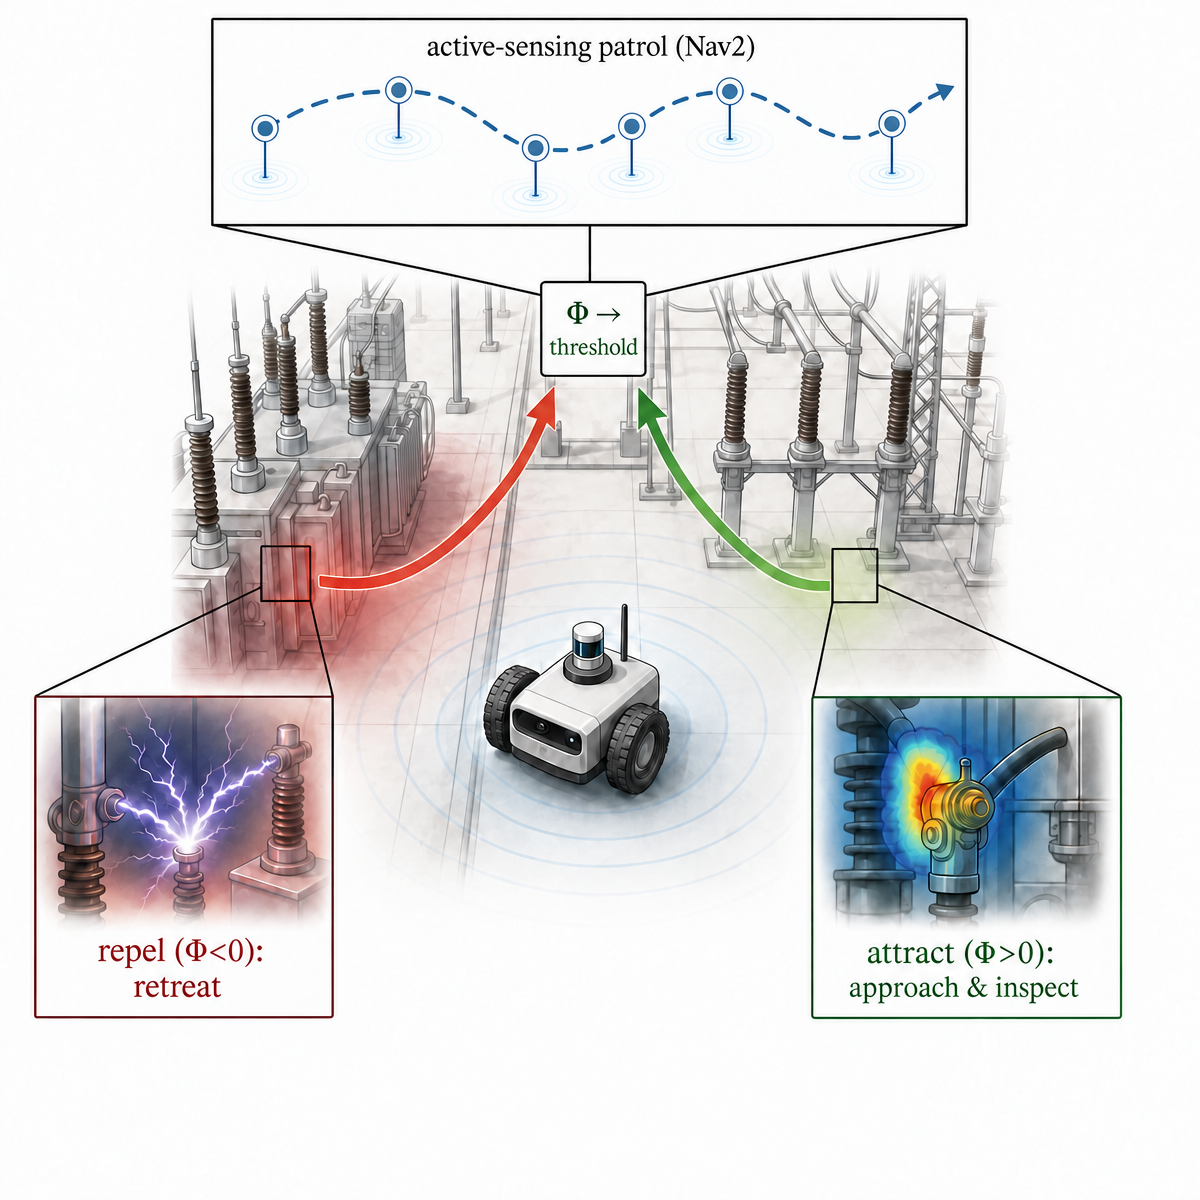
\includegraphics[width=\columnwidth]{concept_overview}
\caption{Concept overview. A deliberative \emph{active-sensing} patrol (Nav2)
carries the robot around the substation, while a \emph{reactive}
layer makes it approach anomalies (attraction) and retreat from hazards
(repulsion) via a threshold on the raw saliency field $\bm{\Phi}$. The same field is
also expressible as an additive term in a tabular value update, recorded as a
design note in Appendix~\ref{app:update} because it does not drive the executed
behavior.}
\label{fig:concept}
\end{figure}

Yet most deployments treat the round as a \emph{fixed coverage} problem: the
robot drives between waypoints and classifies whatever appears, without
adapting its motion to what it senses. The complementary failure mode is the
\emph{purely reactive} controller, which responds only to stimuli already
within sensor range and, in the absence of a stimulus, has nothing to act
upon---besides being prone to local-minima stalls~\cite{koren1991}. What is
missing is a mechanism that (i) carries the sensors to where relevant events may
occur and (ii), once an event is within range, reacts to it---approaching an
anomaly to inspect it, or retreating from a danger.

Our key observation is that these two needs map onto two layers
(Fig.~\ref{fig:concept}). Bringing the
sensors to potential events is a form of \emph{active
sensing}~\cite{bajcsy1988}: the inspection round itself performs this
placement. Reacting to a sensed event is an \emph{affective}
impulse~\cite{breazeal2003}: an attraction toward salient anomalies or a
repulsion from hazards. We realize the second layer as a
threshold-triggered controller driven by a field $\Phi(s)$---positive for
attraction, negative for repulsion, derived from sensory saliency---whose sign
carries a categorical safety precedence. We run this reactive layer on top of a
standard deliberative stack (Nav2 with a Model Predictive Path Integral (MPPI)
controller~\cite{macenski2020nav2,williams2017mppi}), and the deliberative patrol
provides coverage and avoids global stalls.
%% R3#1/R2#1: a menção à equação de Bellman saiu da introdução. O que o sistema
%% avaliado tem é um controlador por limiar; a atualização de valor é registrada
%% como nota de projeto no Apêndice~\ref{app:update}, porque a tabela de valor NÃO
%% seleciona as ações executadas. Prometê-la aqui sugeria um componente de
%% aprendizado inexistente.
For completeness, the same field can be written as an additive term in a tabular
value update; we record that in Appendix~\ref{app:update} as a design note rather
than a mechanism of this system, since the value table does not select the executed
actions and, under a fixed learning rate, the term is equivalent to augmenting the
reward~\cite{ng1999,zhang2023apf}.

We implement the method (named \textsc{Stay Alert}) in ROS~2 with Gazebo and
evaluate it in a simulated substation, comparing the reactive layer against a
fixed baseline patrol and an artificial potential-field baseline, over an
adverse, event-dense scenario and a hazard placed on the patrol route, with
$n=10$ attempted runs per configuration and distribution-free statistical testing. The
reactive layer turns the patrol into an inspection behavior: the baseline
inspects no off-route anomalies, whereas \textsc{Stay Alert} inspects all of them
in the default scenario and performs a consistent hazard-avoidance maneuver, at a
modest increase in mission time ($\approx14\%$ over the fixed baseline) and more
efficiently than the potential-field baseline; inspection completeness degrades
under high perception noise and dense clustering, while no contact-region entries were observed
throughout.

The contributions of this work are as follows:
\begin{itemize}
%% R3#1/R2#1: a lista passou de 4 itens com a formulação de Bellman em destaque para
%% 3 itens organizados por TIPO de contribuição (projeto / avaliação / achados), e
%% não por componente. A atualização de valor saiu da lista e virou nota de projeto
%% no Apêndice~\ref{app:update}. R2-Q3 observou que "arquitetura" e "controlador"
%% se sobrepunham como alegações separadas de novidade.
\item \textbf{The architectural design}: a two-layer scheme that decouples an
\emph{active-sensing} waypoint patrol (Nav2) from a reactive layer whose
attraction/repulsion field drives a threshold-triggered finite-state controller,
arbitrated by a \emph{categorical precedence} rather than a magnitude contest---the
hazard channel governs whenever a hazard is eligible, even when a co-located anomaly
is more salient. The safety response is deliberately two-timescale: a fast reactive
retreat and a persistent deliberative keep-out projected into the global costmap on
detection.

\item \textbf{A comparative evaluation on a standard ROS~2/Nav2 stack} in a simulated
substation (ROS~2 Humble, Nav2/MPPI, Gazebo Fortress). Beyond a fixed patrol and an
artificial potential-field baseline, we add the comparison that isolates the field
itself: a \emph{generic detect--select--deviate--return heuristic driven by raw
detection on the same Nav2/MPPI controller}, plus a one-factor variant that differs
from the proposed layer \emph{only} in the target-selection criterion. We also add a
fixed patrol carrying the same detection-triggered keep-out but no reactive layer,
which is the fair reference for the safety claim. Reporting uses effect sizes,
%% R1 do parecer de verificacao: a contribuicao prometia "confirmatory family
%% stated in advance", que a ressalva da §V contradiz. Os contrastes sao
%% anteriores; o conjunto de desfechos nao.
confidence intervals, distribution-free and equivalence tests, with all fifteen tests
of the primary comparison family reported and Holm-adjusted, retrospective selection
of its outcomes explicitly acknowledged, and everything else labelled exploratory.

\item \textbf{Three attribution and sensitivity findings}, each of which narrows what
may be credited to the proposed layer. (a)~The safety gain on a \emph{static}
on-route hazard is attributable to the detection-triggered keep-out, not to the
reactive weighting: a fixed patrol carrying the same keep-out and no reactive
supervisor reaches a minimum clearance with no detectable difference from the
ablation that keeps the reactive inspection, and what the reactive layer adds is
the inspections. (b)~Replacing saliency by proximity produced no detectable difference in any
scenario, whereas replacing the thresholded field by raw detection---which removes the
hazard channel's temporal persistence---halves the minimum clearance in the co-located
conflict and delays the priority inspection.
(c)~That precedence is not free: a marginally eligible hazard suppresses attraction
for tens of seconds and forfeits one inspection in every run, so the rule buys
clearance at a measurable completeness cost. Code, world, data, and evaluation
scripts are released.
\end{itemize}

The remainder of this article is organized as follows.
Section~\ref{sec:related} reviews related work; Section~\ref{sec:method}
presents the proposed method; Section~\ref{sec:setup} describes the
experimental setup; Section~\ref{sec:results} reports results and discussion;
and Section~\ref{sec:conclusion} concludes.

\section{Related Work}
\label{sec:related}

\subsection{Robotic Inspection of Electrical Substations}
Autonomous ground robots are increasingly deployed to inspect electrical
substations, reducing human exposure to high-voltage hazards while improving
the regularity of meter reading, switch-status recognition and infrared
thermography~\cite{li2024state}. Navigation in this domain must cope
with dense equipment layouts and safety-critical clearances; recent work
improves path planning, e.g., by combining deep reinforcement learning with
ant-colony optimization for substation routing~\cite{zhang2025substation},
reporting gains over deep-RL and classical baselines such as PPO, DDQN, and
A$^{\!*}$; broader surveys catalogue perception and path-planning techniques for
substation mobile robots~\cite{substationpp2024review}. Contemporary substation
systems increasingly couple deep learning with the navigation stack---for example
attention-enhanced semantic segmentation to guide the inspection
robot~\cite{substation2025segnav}, and deep-learning inspection pipelines for
ultra-high-voltage sites~\cite{substation2024uhvdl}. These systems, however,
treat the round as a fixed coverage problem: the robot follows planned routes and
the perception pipeline classifies what is seen.
\emph{In contrast}, we add a reactive affective response \emph{during} the
round, letting saliency steer the robot toward anomalies and away from hazards.

\subsection{Reactive Navigation: Potential Fields and DWA}
Classical reactive methods react to local sensing without a learned value
function. Artificial potential fields (APF) sum attractive and repulsive
forces~\cite{khatib1986} but are well known to stall in local
minima~\cite{koren1991}; the Dynamic Window Approach selects feasible
velocity commands by short-horizon prediction~\cite{fox1997}. Our affective
field $\Phi$ is reminiscent of attraction/repulsion, but the reactive response is
issued by a threshold-triggered controller that preempts the patrol with a goal,
and the deliberative layer prevents the global stalls that afflict pure
potential-field control. We make this comparison concrete by evaluating a
conventional artificial-potential-field controller as a baseline on the same
events (Section~\ref{sec:results}).

\subsection{Reinforcement Learning for Navigation and Reward Shaping}
Reinforcement learning underpins many navigation policies~\cite{suttonbarto2018};
deep reinforcement learning in particular now drives a broad line of map-less and
dynamic-environment navigation, surveyed with its persistent sim-to-real and
safety challenges~\cite{drlrobotics2024survey}. Within this line, \emph{reward
shaping} accelerates learning; potential-based shaping is the canonical form that
preserves the optimal policy~\cite{ng1999}, and shaped rewards have been used for
obstacle avoidance and goal reaching~\cite{zhang2020reward}. A related hybrid line lets RL \emph{tune the
parameters} of an artificial potential field online~\cite{zhang2023apf}. As we
derive in Appendix~\ref{app:update}, writing our field as an additive term in a
value update is, for a fixed learning rate, \emph{equivalent} to augmenting the
reward with a saliency signal; we therefore do not claim it as a new learning
operator, and the architecture evaluated here contains no learning component. What
distinguishes this work is not the term in isolation but the \emph{architecture}:
a saliency-driven attract/repel impulse produced by a reactive layer on top of an
active-sensing patrol, with the value-update formulation offered as a substrate
for future learned policies. The repulsive component and the deliberative
avoidance it triggers also connect to \emph{safe} reinforcement learning, whose
central concern is maintaining safety during learning-driven
control~\cite{brunke2022safe}.

\subsection{Deliberative Stacks: Nav2 and MPPI}
We build the deliberative layer on a mature, reproducible
stack~\cite{macenski2020nav2}, using a Model Predictive Path Integral
controller for path following~\cite{williams2017mppi}. Rather than proposing a
new planner or controller, we keep this layer standard and add the reactive
affective layer on top, so the contribution is orthogonal to (and benefits
from) ongoing improvements in industrial navigation stacks.

\subsection{Active Perception and Affective Robotics}
Active perception holds that perception is purposive: an agent should act to
acquire informative observations~\cite{bajcsy1988}; its modern instantiation is
\emph{informative path planning}, where the robot plans viewpoints to maximize
information gain during mapping and inspection~\cite{ipp2024nonconvex}. Emotion-
and affect-inspired robotics, in turn, models internal drives that bias
behavior~\cite{breazeal2003}. Architecturally, our two layers follow the
classical hybrid deliberative--reactive paradigm, in which a reactive behavior is
arbitrated on top of a deliberative planner~\cite{hybrid2015delibreact}; here the
arbitration is a simple priority (safety before inspection) together with a
saliency threshold. We
connect these threads operationally: the patrol is an \emph{active-sensing} layer
that brings the sensors to where events may occur, and \textsc{Stay Alert} is the
\emph{affective} layer that, once an event is within range, produces an approach
or retreat impulse. Table~\ref{tab:comparison} positions our method against
representative reactive, learning-based, and substation-specific approaches.
Within this scope, we are not aware of a prior method that couples an affective
attraction/repulsion term---formulated in the Bellman update---with an
active-sensing patrol for substation inspection.

\begin{table*}[!t]
\caption{Positioning of the proposed method against representative approaches.
``Active sensing'' denotes moving the platform to acquire observations beyond a
fixed route.}
\label{tab:comparison}
\centering
\footnotesize
\setlength{\tabcolsep}{4pt}
\begin{tabular}{p{2.3cm}p{2.4cm}p{2.7cm}p{1.4cm}p{2.5cm}p{1.7cm}p{2.2cm}}
\hline
\textbf{Method} & \textbf{Learning strategy} & \textbf{Reactive mechanism} &
\textbf{Active sensing} & \textbf{Safety handling} & \textbf{Validation} &
\textbf{Reported metrics} \\
\hline
Classical APF / DWA~\cite{khatib1986,fox1997} & None & Force summation / velocity
search & No & Repulsive force & Sim / analytical & Reach, path length \\
RL-tuned APF~\cite{zhang2023apf} & RL tunes APF gains & Potential field & No &
Repulsive force & Simulation & Success, collisions \\
Substation DRL+ACO~\cite{zhang2025substation} & Deep RL + ant colony & None
(global planner) & No & Planned clearance & Sim + field & Path length, completion
\\
Informative path planning~\cite{ipp2024nonconvex} & Planning (partly learned) &
None & Yes (viewpoints) & Task-dependent & Sim + real & Info.\ gain, coverage \\
\textbf{This work (\textsc{Stay Alert})} & Value augmentation,
threshold-triggered (not learned) & Affective FSM (attract / repel) & Partial:
fixed-patrol sensor exposure + event-triggered repositioning (no informative view
planning) & Reactive retreat + deliberative keepout & Simulation (Gazebo) &
Inspection, safety, mission time (effect sizes, CIs) \\
\hline
\end{tabular}
\end{table*}

\section{Proposed Method}
\label{sec:method}

\subsection{Overview: A Two-Layer Architecture}
\label{sec:method-overview}
The proposed system separates inspection into two cooperating layers
(Fig.~\ref{fig:arch}). A \emph{deliberative} layer performs the inspection
patrol: it visits a sequence of waypoints around the equipment using a standard
navigation stack (Nav2 with a Model Predictive Path Integral controller). We
interpret this layer as \emph{active sensing}: a purely reactive agent responds
only to stimuli already within sensor range, so a mechanism is required
\emph{beforehand} to carry the sensors to where events may occur. The patrol
provides exactly that placement.

A \emph{reactive} layer, named \textsc{Stay Alert}, runs on top of
the patrol. It is governed by an attraction--repulsion field $\Phi$ that grows when a
salient sensory event enters range, driving the robot to \emph{approach}
points of interest (positive $\Phi$, e.g., a thermal hotspot or a partial
discharge) or to \emph{retreat} from danger (negative $\Phi$, e.g., an
arc-flash zone). \textsc{Stay Alert} does not replace the planner: while $\Phi$
is neutral the robot follows the patrol; when an event becomes salient,
\textsc{Stay Alert} preempts the current waypoint, issues a focused navigation
goal (an approach or a retreat pose), and returns control to the patrol once
the event has been handled. This decoupling keeps the deliberative guarantees
of a mature stack while adding a fast, interpretable reactive response.
The field $\Phi$ drives the reactive state machine
(Section~\ref{sec:method-stayalert}); the same field can also be written into a
tabular value update, which we record in Appendix~\ref{app:update} as a design note
since it does not select the executed actions. We revisit this distinction in
Section~\ref{sec:results}.

\begin{figure}[t]
\centering
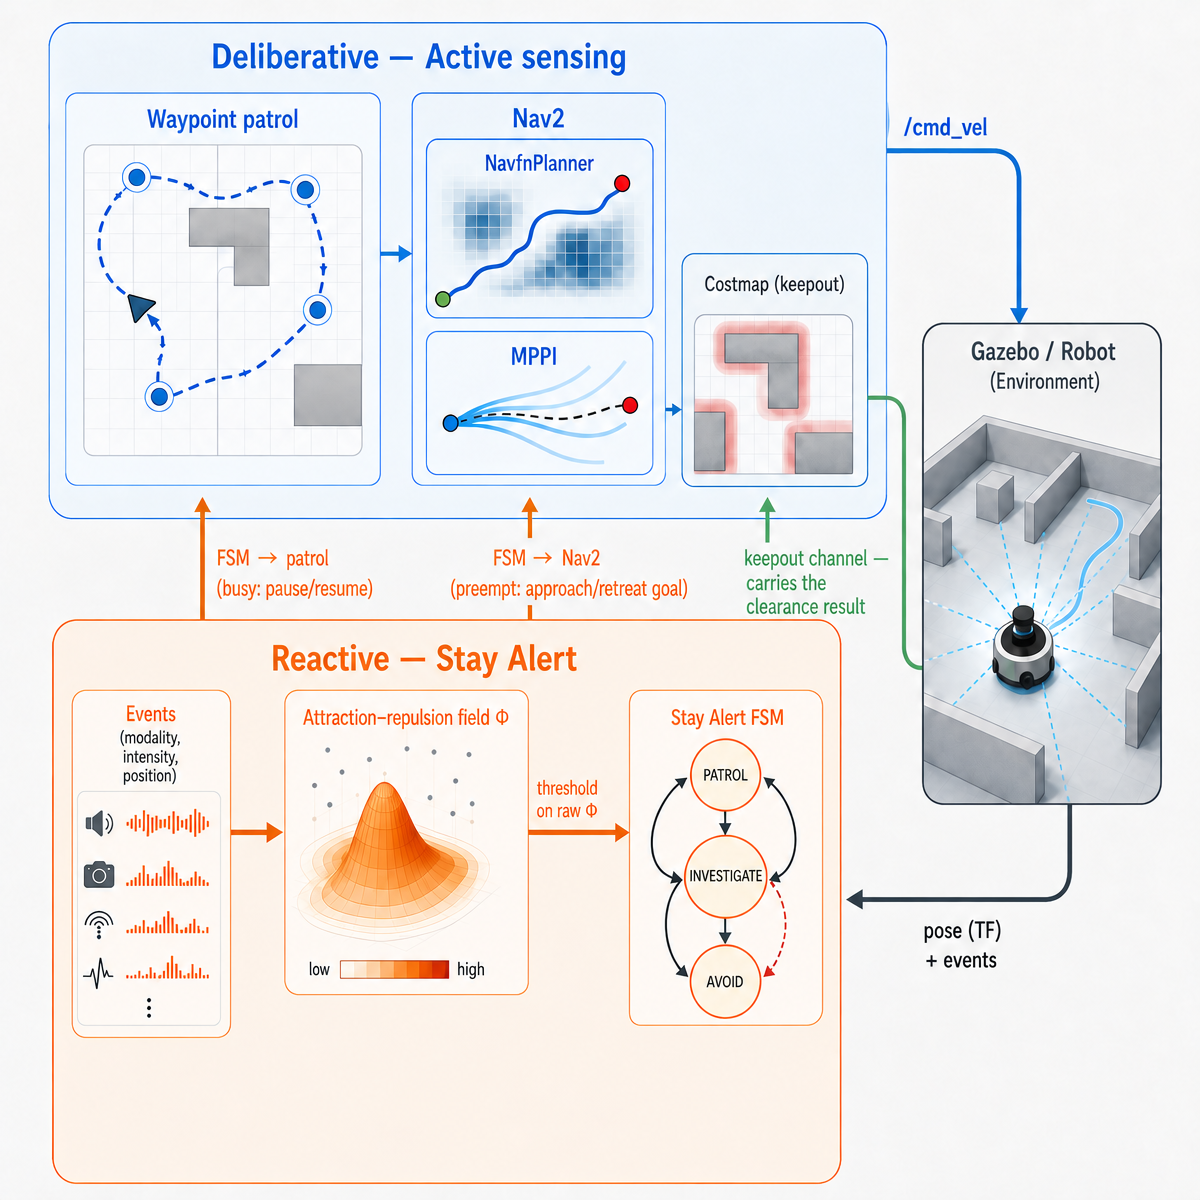
\includegraphics[width=\columnwidth]{architecture}
\caption{Two-layer architecture. The deliberative layer (top) drives a waypoint
patrol through Nav2 (NavfnPlanner $+$ MPPI), sending \texttt{/cmd\_vel} to the
robot. The reactive layer (bottom, \textsc{Stay Alert}) turns sensed
events into the attraction/repulsion field and runs the finite-state machine; it
preempts Nav2 with an approach/retreat goal and pauses/resumes the patrol. The
value update of Appendix~\ref{app:update} is fed by the same field but does not
select the executed actions. The environment returns pose (TF) and events.}
\label{fig:arch}
\end{figure}

\subsection{The Attraction--Repulsion Field}
\label{sec:method-field}
%% R3#1/R2#1 (resubmissão): esta subseção chamava-se "Attractor-Augmented Bellman
%% Update" e abria pela atualização de valor. Como a tabela de valor NÃO seleciona
%% as ações executadas, liderar por ela prometia um componente de aprendizado que o
%% sistema não tem. A subseção passa a definir apenas o que o sistema USA -- o campo
%% e sua arbitragem -- e a formulação da atualização de valor foi movida para o
%% Apêndice~\ref{app:update} como nota de projeto.
The reactive layer is driven by a scalar field $\Phi$ that aggregates the sensory
events at the robot's location---modality, intensity and distance---and carries the
sign of the response: positive for attraction, negative for repulsion. It is a
function of the robot's current observations alone and does not depend on which
action is taken. The field encodes \emph{sensory saliency} and carries the sign of
the response:
\begin{equation}
\label{eq:phi}
\Phi
\begin{cases}
> 0 & \text{attraction (anomaly: approach)}\\
< 0 & \text{repulsion (hazard: retreat)}\\
= 0 & \text{neutral (default patrol behavior).}
\end{cases}
\end{equation}

The field is formed from sensory \emph{events}. An event $e$ of modality
$m\in\{\text{thermal},\text{acoustic},\text{hazard}\}$ at distance $d$ from the
robot is sensed within a detection radius $R$ with intensity
\begin{equation}
\label{eq:intensity}
i_e(d) = I_e\left(1 - \tfrac{1}{2}\,\frac{d}{R}\right), \qquad d \le R,
\end{equation}
$I_e$ being its base intensity. This profile models a \emph{soft detection
boundary}: sensing degrades linearly with range and is not reported beyond $R$.
The resulting step at $d=R$ (from $I_e/2$ to no event) does not induce chattering
of the reactive response, because the controller uses hysteresis---distinct enter
and exit thresholds (Section~\ref{sec:method-stayalert})---and, once it commits to
an event, does not re-select it until the episode ends; an event that lapses at
the boundary therefore cannot repeatedly re-trigger the same maneuver. We further
report the method's sensitivity to perception noise in
Section~\ref{sec:results}. Each modality has a weight $w_m$ (with
$w_{\text{hazard}}<0$ for repulsion) and a trigger threshold $\theta_m$. The
field enforces \emph{safety before inspection} as a \emph{precedence} rule, not a
magnitude contest: whenever any repulsive event is above threshold within range,
$\Phi$ takes its (negative) value; only in the absence of a hazard does the field
select, among the concurrent attraction events, the strongest in magnitude. It
then decays geometrically once the event is no longer observed:
Let $\mathcal{E}_{\mathcal{H}}=\{e:\,m(e)\in\mathcal{H},\ i_e\ge\theta_{m(e)}\}$ and
$\mathcal{E}_{\mathcal{A}}=\{e:\,m(e)\in\mathcal{A},\ i_e\ge\theta_{m(e)}\}$ be the
above-threshold hazard and attraction \emph{events} in range at the current step
(each $e$ carries a modality $m(e)$, intensity $i_e$ and identity). The governing
event and the field are formed by \emph{two decaying accumulators}---a hazard
channel $h\ge 0$ and a signed attraction channel $a$---rather than by a single
instantaneous selection, matching the implementation. Writing $c_e=w_{m(e)}\,i_e$
for the signed contribution of event $e$, each step updates the channels by a
magnitude-preserving max-hold,
\begin{align}
\label{eq:phi-chan}
h &\leftarrow \max\!\big(h,\ \textstyle\max_{e\in\mathcal{E}_{\mathcal{H}}}|c_e|\big),\\
a &\leftarrow c_{e^\star}\ \ \text{when } |c_{e^\star}|>|a|\ \ (\text{else held}),
\end{align}
with $e^\star=\operatorname*{arg\,max}_{e\in\mathcal{E}_{\mathcal{A}}}|c_e|$ and
ties broken by the smallest event identity. Once per decay period both channels
relax geometrically and are floored at a residual $\varepsilon$,
\begin{equation}
\label{eq:phi-decay}
h\leftarrow\lambda h,\qquad a\leftarrow\lambda a\quad(\text{set to }0\text{ if below }\varepsilon).
\end{equation}
Each accumulator is \emph{saturated in place} on update---$h\in[0,\Phi_{\max}]$
and $a\in[-\Phi_{\max},\Phi_{\max}]$---so the stored value, not merely its
reading, is bounded (the decay of Eq.~\eqref{eq:phi-decay} then acts on this
bounded state). The field is read off by \emph{categorical precedence},
\begin{equation}
\label{eq:phi-update}
\Phi=-h\ \ \text{if } h>\varepsilon,\qquad
\Phi=a\ \ \text{otherwise,}
\end{equation}
with decay $\lambda\in(0,1)$, residual $\varepsilon$, decay period $T_d$, and
$\mathcal{H}$, $\mathcal{A}$ indexing the repulsive and attractive modalities; when
a channel's \emph{own} eligible set is empty at a step, that channel is left to the
decay of Eq.~\eqref{eq:phi-decay} while the other may still be updated by its
events. We use $\lambda=0.85$, $T_d=1$~s,
$\varepsilon=10^{-3}$ and $\Phi_{\max}=2$ (Table~\ref{tab:hyper}). This memory has two consequences a purely
instantaneous rule would lack: (i) a \emph{recently observed} hazard keeps
governing the field through its decaying magnitude even when only an attraction is
in range at the current step, until $h$ falls below $\varepsilon$; and (ii) a
weaker current event does not overwrite a stronger stored one until the latter has
decayed. Hazards are considered first, so a hazard channel above $\varepsilon$
always governs the field, independently of a concurrent stronger attraction: the
magnitude contest only ever decides \emph{which anomaly} to approach, never
whether to prefer inspection over safety. The \textsc{Avoid} transition then fires
when this field crosses the supervisor threshold ($\Phi\le-\theta_{\text{in}}$)
\emph{and} a retreat pose is available, the post-retreat refractory has elapsed,
and the reactive retreat is enabled (Algorithm~\ref{alg:stayalert})---not as a
function of hazard range alone. We verify the precedence directly in a conflict
scenario (Section~\ref{sec:conflict}), in which a hazard co-located with a
\emph{stronger} anomaly still preempts inspection.

\subsection{The \textsc{Stay Alert} Reactive Layer}
\label{sec:method-stayalert}
\textsc{Stay Alert} is a finite-state machine with three modes:
\textsc{Patrol}, \textsc{Investigate} (attraction) and \textsc{Avoid}
(repulsion), summarized in Algorithm~\ref{alg:stayalert} and
Fig.~\ref{fig:fsm}. Repulsion has priority over attraction (safety before
inspection) \emph{from any state}: whenever $\Phi \le -\theta_{\text{in}}$ and a
retreat pose is available, the robot enters \textsc{Avoid} and navigates to a
retreat pose---\emph{preempting} an in-progress \textsc{Investigate} (outcome
\emph{deferred})---subject to a short refractory $t_{\text{ref}}$ that prevents
immediate re-triggering while the deliberative keepout (Section~\ref{sec:results})
takes over. Otherwise, from \textsc{Patrol}, if $\Phi \ge \theta_{\text{in}}$ the
layer commits the most salient in-range event and enters \textsc{Investigate},
navigating to its inspection pose. On entering either mode the layer asserts a
\emph{busy} flag that pauses the patrol (the current waypoint goal is cancelled)
and emits an event marker carrying the target's identity.

\textsc{Investigate} terminates \emph{successfully} (outcome \emph{inspected})
only when the reactive navigation \emph{succeeds}, the controller holds for a
commanded dwell $t_{\text{dwell}}$, and the simulator confirms the final pose lies
within a \emph{confirmation distance} of the \emph{true} target (the standoff plus
a tolerance; Section~\ref{sec:setup-matrix}); a navigation that is aborted or
cancelled, or a budget $t_{\max}$ that elapses, ends the episode as \emph{failed}.
This confirmation is a proxy---it does not independently verify the full standoff
and orientation, nor persistence throughout the dwell---and we name the metric
accordingly. It does
\emph{not} exit merely because $\Phi$ decayed, which prevents oscillation while
crossing a low-saliency ``valley'' between events. \textsc{Avoid} terminates when
the hazard leaves range, $\Phi > -\theta_{\text{out}}$ (\emph{safe}), or upon
reaching the retreat pose (\emph{retreated}), and then arms the refractory. On any
exit the busy flag is released and the patrol resumes the \emph{same} waypoint. An
anomaly is \emph{committed} at the \emph{start} of its investigation---after which
it stops attracting, removing the
\textsc{Patrol}$\leftrightarrow$\textsc{Investigate} oscillation that arises when a
waypoint lies close to an anomaly---and is counted as \emph{inspected} only on a
confirmed successful arrival. Episodes that end in \emph{failed} (timeout/abort) or
\emph{deferred} (hazard preemption) are kept as distinct outcomes and never counted
as inspections; we report commits, inspections, failures, and deferrals separately
(Section~\ref{sec:results}).

\paragraph*{Deliberative keepout} A hazard on the patrol route cannot be resolved by
a reactive retreat alone, since the next waypoint lies beyond it. We therefore add a
\emph{deliberative} expression of the repulsion: whenever a hazard is \emph{detected}
within sensor range, its \emph{perceived} position is projected as a \emph{persistent}
keepout region into the global costmap, which the planner then routes around for the
remainder of the mission. This projection is a map channel driven by detection---not
a consequence of completing a retreat---and it uses the same perceived information as
the reactive layer. When a reactive retreat does fire, the hazard is additionally
\emph{handed off} to this channel: its reactive signal $\Phi$ is suppressed, so the
robot does not oscillate between retreating and re-approaching while the planner
contours the mark. The safety outcomes we report (clearance, time-to-collision,
contact-region entries) are measured throughout from the hazard's \emph{true}
position, independently of $\Phi$, so suppressing the reactive signal does not
inflate them.

\begin{figure}[t]
\centering
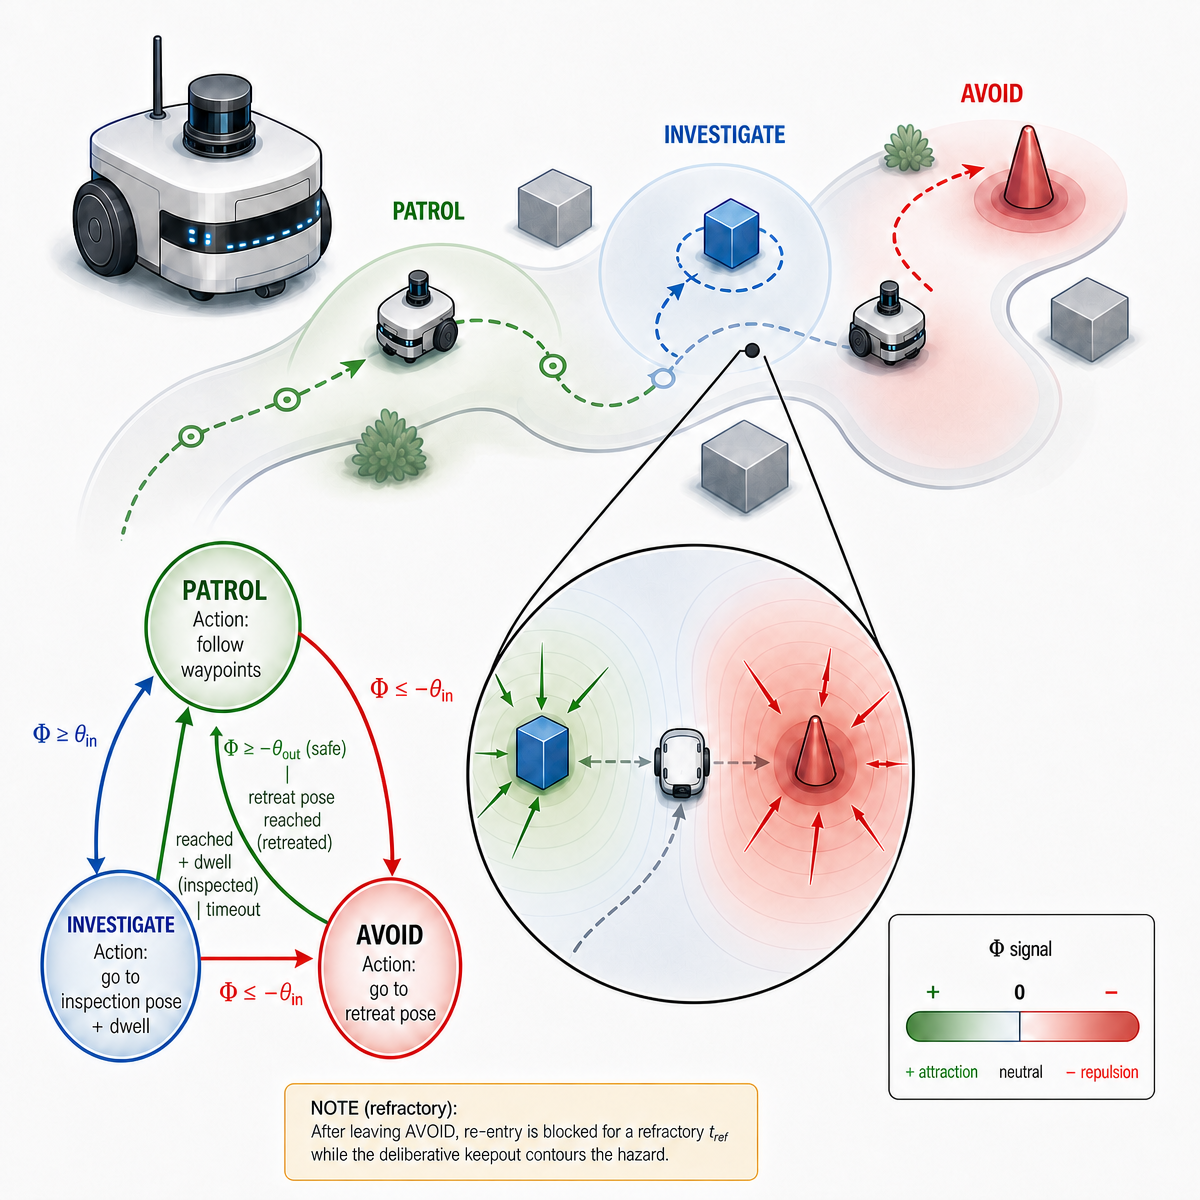
\includegraphics[width=\columnwidth]{stay_alert_fsm}
\caption{\textsc{Stay Alert} state machine and attraction--repulsion field. Top: along the
patrol the robot switches to \textsc{Investigate} (approach an anomaly) or
\textsc{Avoid} (retreat from a hazard). Bottom-left: the three modes and their
transitions ($\theta_{\text{in}},\theta_{\text{out}}$ thresholds; outcomes
\emph{inspected}/\emph{timeout}/\emph{safe}/\emph{retreated}; repulsion has
priority). Bottom-right: the field pulls toward attraction (green) and
pushes away from repulsion (red).}
\label{fig:fsm}
\end{figure}

\begin{algorithm}[t]
\caption{\textsc{Stay Alert} reactive layer (per control tick)}
\label{alg:stayalert}
\begin{algorithmic}[1]
\STATE \textbf{input:} field $\Phi$; selected event $e^\star$ (most salient in
       range); thresholds $\theta_{\text{in}},\theta_{\text{out}}$;
       $t_{\text{dwell}}, t_{\max}$; refractory $t_{\text{ref}}$
\STATE \textbf{Safety preemption} (a hazard interrupts \emph{any} state):
\IF{mode $\ne$ \textsc{Avoid} \textbf{and} $\Phi \le -\theta_{\text{in}}$
    \textbf{and} retreat pose available \textbf{and} $t \ge t_{\text{avoid}}$}
  \IF{mode $=$ \textsc{Investigate}}
     \STATE exit (\emph{deferred by hazard}); release target $e^\star$
  \ENDIF
  \STATE enter \textsc{Avoid}; pause patrol; send retreat goal; \emph{hand the
         hazard to the deliberative keepout} (its reactive signal is thereafter
         suppressed, to avoid oscillation while the planner contours it)
\ELSIF{mode $=$ \textsc{Patrol}}
  \IF{$\Phi \ge \theta_{\text{in}}$ \textbf{and} inspection pose available}
     \STATE commit target $e^\star$ (by identity); enter \textsc{Investigate};
            pause patrol; send approach goal
  \ENDIF
\ELSIF{mode $=$ \textsc{Investigate}}
  \IF{navigation \textbf{succeeded}, dwelled $\ge t_{\text{dwell}}$, \textbf{and}
      final pose within the confirmation distance of $e^\star$}
     \STATE exit (\emph{inspected}: credit $e^\star$); resume patrol
  \ELSIF{elapsed $\ge t_{\max}$ \textbf{or} navigation aborted/cancelled}
     \STATE exit (\emph{failed}); resume patrol
  \ENDIF
\ELSIF{mode $=$ \textsc{Avoid}}
  \IF{$\Phi > -\theta_{\text{out}}$ \textbf{or} retreat pose reached}
     \STATE exit (\emph{safe}/\emph{retreated});
            $t_{\text{avoid}} \gets t + t_{\text{ref}}$; resume patrol
  \ELSIF{elapsed $\ge t_{\max}$}
     \STATE exit (\emph{timeout});
            $t_{\text{avoid}} \gets t + t_{\text{ref}}$; resume patrol
  \ENDIF
\ENDIF
\end{algorithmic}
\end{algorithm}

\subsection{Active Sensing and Event Abstraction}
\label{sec:method-sensing}
The patrol realizes active sensing by carrying the sensors along the route; the
robot pose used by the reactive layer is taken in the \emph{map} frame (via the
TF tree), so that events, poses and the static map are mutually consistent. The
output of the sensing-and-perception chain is abstracted as \emph{events}
$(\text{modality}, \text{intensity}, \text{position})$, i.e., we model the
\emph{result} of perception rather than raw sensor streams. This is a scoped
simplification appropriate to an \emph{algorithmic} contribution: it isolates
the navigation-and-decision behavior from the (orthogonal) perception problem,
and keeps the evaluation reproducible.

Given an event at position $\bm{e}$ and the robot at $\bm{p}$, with unit
direction $\hat{\bm{u}}=(\bm{p}-\bm{e})/\lVert\bm{p}-\bm{e}\rVert$,
\textsc{Investigate} targets an inspection pose at a standoff $\rho$ facing the
event, $\bm{p}_{\text{insp}}=\bm{e}+\rho\,\hat{\bm{u}}$, while \textsc{Avoid}
targets a retreat pose beyond the detection radius and facing away,
$\bm{p}_{\text{ret}}=\bm{e}+(R+\Delta)\,\hat{\bm{u}}$. Attraction events are
committed once (then stop attracting); hazards are persistent.

\section{Experimental Setup}
\label{sec:setup}

\subsection{Simulation Environment and Software Stack}
\label{sec:setup-stack}
Experiments run on ROS~2 Humble with Gazebo Fortress (Ignition Gazebo~6) as the
physics simulator, bridged through \texttt{ros\_gz}. The robot is a
differential-drive platform (\emph{inspector\_bot}) with a 360$^\circ$ planar
range sensor. Global path planning uses the Nav2 stack with the
\emph{NavfnPlanner} global planner and a Model Predictive Path Integral (MPPI)
controller for path following (differential motion model, control frequency
$20$~Hz) over a \emph{static} occupancy map. The Nav2 stack is configured with
Adaptive Monte Carlo Localization (AMCL), but in these experiments the
map$\rightarrow$odom transform is held fixed so that the robot pose is exact and
localization drift is not modeled (its treatment is left as future work,
Section~\ref{sec:setup-repro}); the pose used by the perception and metrics nodes
is therefore the ground-truth map-frame transform, not an AMCL estimate. The
costmaps use a robot radius of $0.25$~m, an
inflation radius of $0.55$~m and a cost-scaling factor of $3.0$; the goal
tolerance is $0.25$~m.

The world models a simplified substation (Fig.~\ref{fig:world}): a power
transformer ($3{\times}2{\times}1.5$~m at $(10,10)$), a circuit breaker
($1{\times}1{\times}2$~m at $(-5,5)$), a busbar ($8{\times}0.3{\times}0.3$~m at
$(0,15)$) and a $50{\times}50$~m perimeter fence, on a ground plane. The static
occupancy map ($1040{\times}1040$ cells at $0.05$~m/cell) is aligned with the
world frame, so waypoints in world coordinates serve directly as navigation
goals. The deliberative patrol visits five waypoints
(in metres): $(13,-8)$, $(13,10)$, $(0,11)$, $(-8,5)$ and a return at
$(-10,-10)$.

\begin{figure}[t]
\centering
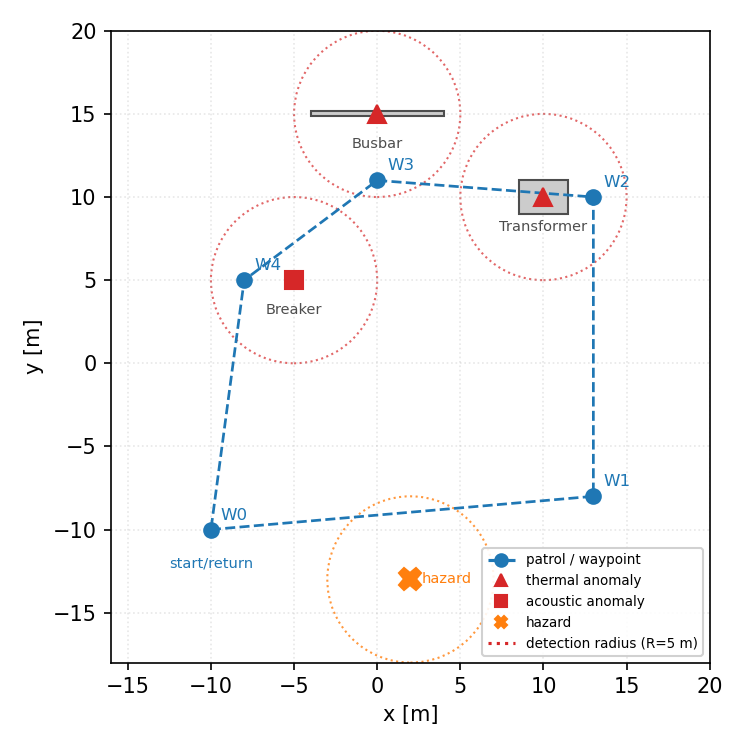
\includegraphics[width=\columnwidth]{world_map}
\caption{Substation scenario (default): equipment (gray), the five patrol
waypoints W0--W4 and the round (dashed), the attraction anomalies (thermal
$\triangle$, acoustic $\square$) and the hazard ($\times$), each with its
$R=5$~m detection radius (dotted). Coordinates in metres, world frame.}
\label{fig:world}
\end{figure}

\subsection{Simulated Events}
\label{sec:setup-events}
Following Section~\ref{sec:method-sensing}, the perception output is abstracted
as events. The \emph{default} scenario has three attraction anomalies --- a
thermal event at the transformer $(10,10)$, a thermal event at the busbar
$(0,15)$ and an acoustic event at the breaker $(-5,5)$ --- and one persistent
hazard (repulsion) beside the first patrol leg at $(2,-13)$. The \emph{adverse}
scenario (E5) densifies the anomalies into clusters (five anomalies: two near
the transformer and two near the breaker, plus the busbar), so that multiple
events fall within the sensory radius simultaneously and the layer must
arbitrate between them; the hazard is unchanged. The \emph{route-hazard} scenario
(RHM/RHB) keeps the three default anomalies but moves the hazard \emph{onto} the
first patrol leg at $(1.5,-9)$---directly blocking the path to the next
waypoint---so that a purely reactive retreat cannot resolve it without deviating
the route; here the detected hazard is also projected, at its \emph{perceived}
position, as a \emph{persistent} keepout into the global costmap (a mark the
deliberative planner routes around for the rest of the mission). The \emph{conflict} scenario
(CONF) keeps the three default anomalies and co-locates, at the default hazard's
position $(2,-13)$, a \emph{strong} acoustic anomaly ($I_e=0.95$,
$|w\,I_e|=1.14$) with a \emph{weaker} hazard ($I_e=0.70$, $|w\,I_e|=1.05$): the
attraction is the more salient of the two, so a magnitude-only rule would prefer
inspection, whereas the precedence rule must trigger \textsc{Avoid}. The
detection radius is $R=5$~m, the inspection standoff $\rho=2$~m and the retreat
margin $\Delta=1.5$~m (full coordinates and intensities in
Appendix~\ref{app:params}).

\subsection{Experimental Matrix and Metrics}
\label{sec:setup-matrix}
We evaluate the affective layer against a fixed baseline and an
artificial-potential-field baseline, across an $\eta$ sweep, an $\eta=0$ (affective-value) ablation,
an adverse scenario, a hazard placed on the route, and perception-noise
perturbations (Table~\ref{tab:matrix}); each configuration is run $n=10$ times
(headless, $600$~s timeout per run). \textbf{E1} is the deliberative patrol
\emph{without} the reactive layer (no affective response). \textbf{E0} is an
ablation that enables \textsc{Stay Alert} but sets the value-update weight
$\eta=0$. \textbf{E2--E4} enable the full method with
$\eta\in\{0.3,0.5,0.8\}$, and \textbf{E5} uses $\eta=0.5$ on the adverse
scenario. \textbf{APF} replaces the reactive layer with a conventional
artificial-potential-field controller acting on the same events. \textbf{RHM}
and \textbf{RHB} place the hazard \emph{on} a patrol leg---for the method (with
the detected hazard projected as a persistent deliberative keepout) and for
the fixed baseline, respectively. \textbf{N1} and \textbf{N2} repeat the method
under moderate and high zero-mean Gaussian perception noise on event position and
intensity. \textbf{CONF} co-locates a strong attraction event with a weaker
hazard (Section~\ref{sec:setup-events}) to test whether the safety precedence of
Eq.~\eqref{eq:phi-update} holds when both event types are simultaneously within
range. \textbf{KOa} and \textbf{KOb} ablate the on-route safety response into its
two mechanisms---keepout only (reactive retreat disabled) and retreat only
(deliberative keepout disabled)---so that RHM (both), KOa, and KOb isolate the
contribution of each to passing an on-route hazard. \textbf{DHa} and \textbf{DHb}
run a \emph{directed} test of the reactive retreat's transient value: in the
\emph{dyn-hazard} scenario a hazard is co-located with an anomaly and stays
\emph{inactive} until the robot---already committed to inspecting it---closes to
$3$~m, at which point it activates (the environment decides when the hazard
appears). DHa enables the reactive retreat (with keepout) and DHb disables it
(keepout only), isolating what the retreat adds when a hazard \emph{emerges during}
an investigation, a case the static scenarios cannot exercise. The method and
simulation hyperparameters are summarized in Table~\ref{tab:hyper}.

\begin{table}[t]
\centering
\caption{Experimental matrix ($10$ attempted runs each).}
\label{tab:matrix}
\begin{tabular}{llccc}
\hline
\textbf{Exp.} & \textbf{Reactive layer} & $\bm{\eta}$ & \textbf{Scenario} &
\textbf{\#anom./haz.}\\
\hline
E1  & none                 & --   & default      & 3 / 1\\
E0  & Stay Alert (ablation)& 0    & default      & 3 / 1\\
E2  & Stay Alert           & 0.3  & default      & 3 / 1\\
E3  & Stay Alert           & 0.5  & default      & 3 / 1\\
E4  & Stay Alert           & 0.8  & default      & 3 / 1\\
E5  & Stay Alert           & 0.5  & adverse      & 5 / 1\\
APF & potential field      & --   & default      & 3 / 1\\
RHM & Stay Alert           & 0.5  & route-hazard & 3 / 1\\
RHB & none                 & --   & route-hazard & 3 / 1\\
N1  & Stay Alert (noise m.)& 0.5  & default      & 3 / 1\\
N2  & Stay Alert (noise h.)& 0.5  & default      & 3 / 1\\
CONF& Stay Alert           & 0.5  & conflict     & 4 / 1\\
KOa & keepout only         & 0.5  & route-hazard & 3 / 1\\
KOb & retreat only         & 0.5  & route-hazard & 3 / 1\\
DHa & retreat $+$ keepout  & 0.5  & dyn-hazard   & 1 / 1\\
DHb & keepout only         & 0.5  & dyn-hazard   & 1 / 1\\
\hline
\end{tabular}
\end{table}

Each run is logged by a metrics node and reduced to its final values. We report:
\emph{anomalies inspected} (unique, credited only when the reactive navigation
\emph{succeeds}, a commanded dwell of $t_{\text{dwell}}$ elapses, and the simulator
confirms the robot's final pose lies within a \emph{confirmation distance} of the
\emph{true} target---the standoff plus a tolerance, $\rho + 1.3 = 3.3$~m; the dwell
is enforced by the controller rather than independently verified, so this metric
measures \emph{confirmed arrival within $3.3$~m plus a commanded dwell}, a proxy for
physical inspection, not the full standoff-and-orientation condition);
\emph{investigation time}; \emph{route deviations} (affective triggers);
\emph{hazard avoidances} (retreat events); \emph{minimum hazard distance}
(closest approach to a hazard, higher is better); and, for the on-route hazard,
safety-oriented \emph{proxies} computed from the true hazard position:
\emph{contact-region entries} (``collisions''; centre-to-centre distance below
$0.5$~m, a simulated proxy rather than a physical contact sensor), \emph{time below
a clearance threshold} ($2$~m, centre-to-centre), \emph{minimum radial
time-to-collision}
($d/\dot d$ to the nearest hazard, an approaching-rate proxy, not a
trajectory-intersection time), and \emph{retreat success}; \emph{mission duration};
\emph{distance travelled}; and the complete value-update residual
$|\alpha\delta+\eta\Phi|$ as a stability proxy. Because several outcomes are
bounded counts with (near-)zero variance, group comparisons use distribution-free
%% Nomenclatura dos instrumentos geometricos: ambos sao ENTRADAS EM REGIAO
%% definida operacionalmente por distancia, nao contato fisico nem distancia
%% regulamentar. Sem a calibracao pelo raio do robo o leitor nao consegue julgar o
%% que 0.5 m significa.
Both geometric safety instruments are entries into regions defined operationally by
centre-to-centre distance, counted on the rising edge, and computed against the
\emph{true} hazard position with the robot pose taken from the \texttt{map} frame.
Neither is a physical contact measurement, and neither is a regulatory electrical
clearance. To let the reader calibrate them: the robot radius configured in the
planner is $0.25$~m, so the $0.5$~m contact region corresponds to the robot body
reaching the hazard centre, and the $2$~m band to $1.75$~m of clearance from the
robot's edge. The $2$~m value is a diagnostic threshold adopted for measuring
exposure in this evaluation; the study declares no minimum-clearance requirement, so
transiting below it is not a requirement violation but an exposure that we report.

tests (Mann--Whitney $U$, exact for untied samples with $n_1+n_2\le20$ and by
permutation for degenerate arms; see Section~\ref{sec:results}) with the Cliff's
$\delta$ effect size, $95\%$ bootstrap confidence intervals, numeric $p$-values,
and Holm correction across the confirmatory family; equivalence claims use a two
one-sided test (TOST) against a pre-declared margin, and per-mission success rates
use Wilson-score intervals. Runs in which the platform failed to initialize are
excluded as a startup-reliability outcome.

\begin{table}[t]
\centering
\caption{Method and simulation hyperparameters.}
\label{tab:hyper}
\begin{tabular}{lll}
\hline
\textbf{Group} & \textbf{Parameter} & \textbf{Value}\\
\hline
Value update & learning rate $\alpha$ & 0.1\\
(App.~\ref{app:update}) & discount $\gamma$ & 0.95\\
          & affective weight $\eta$ & 0.3 / 0.5 / 0.8\\
          & cell size $\delta$; buckets $B$ & 1.0~m; 4\\
          & progress reward $r_{\text{prog}}$ & 1.0\\
Field $\Phi$ & weights (therm./acou./haz.) & 1.0 / 1.2 / $-1.5$\\
          & thresholds $\theta_m$ & 0.4 / 0.3 / 0.3\\
          & decay $\lambda$; clip $\Phi_{\max}$ & 0.85; 2.0\\
          & decay period $T_d$; residual $\varepsilon$ & 1~s; $10^{-3}$\\
\textsc{Stay Alert} & enter $\theta_{\text{in}}$; exit $\theta_{\text{out}}$ & 0.45; 0.25\\
          & dwell $t_{\text{dwell}}$; budget $t_{\max}$ & 3~s; 40~s\\
          & refractory $t_{\text{ref}}$ & 8~s\\
Evaluator & confirm.\ distance (metric) & 3.3~m\\
Keepout   & project radius; disc radius & 5~m; 1.2~m\\
APF base. & standoff; budget & 1.8~m; 30~s\\
Events    & radius $R$; standoff $\rho$ & 5~m; 2~m\\
          & retreat margin $\Delta$ & 1.5~m\\
\hline
\end{tabular}
\end{table}

\subsection{Reproducibility}
\label{sec:setup-repro}
The full code, world, launch files, the batch runner and the analysis script
are publicly available\footnote{\texttt{github.com/voidmmn/tese\_react\_nav}}.
Installation scripts set up ROS~2
Humble, Gazebo Fortress and Nav2; a batch script runs the full matrix
and writes one CSV per run, and the analysis script produces the summary table,
the effect-size and distribution-free comparisons, and the boxplots (the boxplot
and value-residual figures are produced by released scripts). Alongside the
per-run CSVs of aggregate counts, we release a \emph{consolidated per-episode
audit trail} (\texttt{audit\_trail.csv}), regenerated by a released script from the
per-episode log messages of both the evaluator and the supervisor. Each row is
keyed by configuration, run seed and episode, and carries: for an investigation,
the target identity and its \emph{true} position, and the outcome---the confirmed
arrival distance (\emph{inspected}), a confirmation \emph{rejected} with its
distance and threshold, an \emph{inspection\_failed} with its cause
(timeout / navigation), or \emph{deferred}; for the reactive avoid, its entry, its
exit reason (\emph{safe} / \emph{retreated} / \emph{timeout}), and the reactive
navigation goal's \emph{nav\_result} (aborted / cancelled / rejected); and, for the
dynamic-hazard scenario, the hazard-activation instant (in simulation time) and the
first keepout and reactive publications with the robot pose. The schema keeps the
target's true position and the robot's pose in \emph{separate} columns and records
both the simulation time (where the message carries it) and the log timestamp.
From this trail the confirmation rejections, the inspection failures, and the avoid
outcomes reported throughout Section~\ref{sec:results} (the dynamic-hazard,
adverse and perception-noise analyses) are auditable per episode; its
investigation, credit, deferral and \textsc{Stay Alert} avoid counts cross-check
the corresponding aggregate CSVs. The avoid-event extraction covers the
\textsc{Stay Alert} supervisor; the APF baseline logs its avoidances through a
different path, so those events are counted in the aggregate CSVs but not itemized
in the trail. Experiments
ran on a workstation (Intel Xeon W-1350, 12~cores, 16~GB RAM) under Ubuntu~22.04
(WSL2), headless, at a near real-time factor ($\mathrm{RTF}\approx1$); the
perception-noise generator is seeded \emph{per repetition} (the run index is passed
as the seed and recorded in each CSV), while the remaining run-to-run variation is
the inherent stochasticity of the physics simulator and of the timing in the
navigation stack. The exact code version that produced the
reported results is archived under the tagged release
\texttt{v1.0-resubmission} in the repository. Three configurations---the dense
scenario E5 and the two dynamic-hazard trials DHa and DHb---were re-run under the
corrected hazard-activation and failure-handling code; the other thirteen were
reused. This reuse is a \emph{verifiable identity}, not an assumption: those
thirteen record zero navigation aborts, cancellations, and rejections, so the
corrected failure-handling path is never exercised in them and their metrics are
unchanged under either version, as their published counters show. A provenance
manifest (\texttt{PROVENANCE.md}) records the reference snapshot for each batch, the
per-run seeds, and SHA-256 checksums of all $160$ CSVs, and identifies the replaced
files; the mobile tag alone does not fix this correspondence. As the contribution is the affective
navigation policy operating on abstracted events, it does not depend on raw range
data: obstacle geometry is provided by the static map, and the odometry is kept
exact (the map$\rightarrow$odom transform is held fixed), so we do \emph{not}
model localization drift here; robustness to localization error, event
persistence, and map geometry is left as future work, complementing the
perception-noise sweep of Section~\ref{sec:robustness}.

\section{Results and Discussion}
\label{sec:results}
We report the final per-run values of each metric, aggregated over up to $n=10$
runs per configuration (Table~\ref{tab:results}). Because several outcomes are
bounded counts with (near-)zero variance---for which the assumptions of a
parametric $t$-test do not hold---group comparisons use distribution-free tests
(Mann--Whitney $U$, whose $p$ is computed by case: the \emph{exact} $U$
distribution for untied samples with $n_1+n_2\le20$ (all pairs here), a
two-sided exact permutation $p$ for fully separated constant arms, and the
tie-corrected normal approximation only when ties are present), reported with the
Cliff's $\delta$ effect size and $95\%$ bootstrap confidence intervals, with
numeric $p$-values Holm-corrected across the confirmatory family; equivalence is
assessed by a two one-sided test (TOST) and per-mission success by Wilson-score
intervals.
Runs in which the platform did not move
(travelled distance $\approx 0$) are a startup-reliability
outcome rather than a navigation result: of the $160$ attempted runs, $154$ met the
movement criterion for behavioral analysis and $6$ remained immobile. The
observable, published criterion for these six is \emph{immobility} (the analyzer's
distance criterion; most carry an accumulated mission clock but no motion); we read
them as consistent with an \emph{initialization} failure (the navigation container
not bringing the robot up), rather than the mid-mission timeouts of the earlier
submission, but do not certify that infrastructure cause from published raw logs. We report two complementary views rather than pooling them:
(i) performance \emph{conditional on successful initialization}, computed on the
valid runs ($n=8$--$10$ per configuration); and (ii) \emph{per-attempt} startup
reliability ($154/160=96.25\%$). We do \emph{not} average the immobile runs into
the behavioral metrics---their zero distance and zero inspection would bias the
means and rates---but report them separately as the reliability outcome; the
per-run values (with per-run seeds and outcomes) are released with the code.
%% R2#4: "the boundary between confirmatory and exploratory claims is not always
%% easy to trace through the narrative". Declaracao explicita da familia, e cada
%% alegacao no texto passa a dizer de qual familia vem.
\paragraph*{Confirmatory and exploratory claims} We fix the boundary here and mark it
at every claim rather than only in the tables. The \emph{confirmatory} family,
specified before the new runs were executed, contains three comparisons in the
scenarios they were designed for: the proposed layer against the generic heuristic
and against the one-factor selection variant in the \texttt{default} scenario, and
the keep-out-only ablation against the fixed patrol carrying the same keep-out
(KOa vs.\ KOF) on the on-route hazard. Those are Holm-corrected within the family and
are reported with $p_{\mathrm{Holm}}$. Everything else---the \texttt{conflict} and
\texttt{adverse} scenarios, the threshold and hysteresis sweeps, the marginal-hazard
configuration, and every re-analysis of previously recorded runs---is
\emph{exploratory}, is reported with uncorrected $p$, and is labelled as exploratory
in the sentence that states it. Two of the analyses below are additionally
\emph{retrospective}: the confirmation-distance re-scoring and the boundary-crossing
count operate on runs recorded for the earlier submission, and are planned now rather
than in advance.

The principal (confirmatory) comparisons are consolidated in
Table~\ref{tab:stats}; the remaining equivalence, noise-robustness, and
adverse-cost comparisons are reported in Appendix~\ref{app:stats}
(Table~\ref{tab:allstats}).

\begin{table*}[t]
\centering
\caption{Consolidated statistics for the principal comparisons (valid runs).
$\Delta$ is the mean difference (second minus first configuration); $\delta$ is
Cliff's effect size; the CI is the $95\%$ bootstrap interval of $\Delta$; $p$ is
the Mann--Whitney $U$ (exact $U$ distribution for untied samples with
$n_1+n_2\le20$; exact permutation for fully separated constant arms; tie-corrected
normal approximation when ties are present); $p_{\mathrm{H}}$ is Holm-corrected
across the family.}
\label{tab:stats}
\footnotesize
\setlength{\tabcolsep}{5pt}
\begin{tabular}{llccccc}
\hline
\textbf{Pair} & \textbf{Metric} & $\bm{\Delta}$ & $\bm{\delta}$ & \textbf{95\% CI} & $\bm{p}$ & $\bm{p_{\mathrm{H}}}$\\
\hline
E1 vs E3   & Anomalies inspected   & $+3.00$ & $+1.00$ & $[+3.00,+3.00]$ & $1.1{\times}10^{-5}$ & $7.6{\times}10^{-5}$\\
E1 vs E3   & Min.\ hazard dist.\ [m] & $+0.15$ & $+1.00$ & $[+0.13,+0.17]$ & $1.1{\times}10^{-5}$ & $7.6{\times}10^{-5}$\\
E1 vs E3   & Mission time [s]      & $+44$   & $+1.00$ & $[+43,+45]$     & $1.8{\times}10^{-4}$ & $1.8{\times}10^{-4}$\\
E3 vs APF  & Mission time [s]      & $+39$   & $+1.00$ & $[+36,+42]$     & $2.2{\times}10^{-5}$ & $1.1{\times}10^{-4}$\\
RHB vs RHM & Anomalies inspected   & $+3.00$ & $+1.00$ & $[+3.00,+3.00]$ & $2.2{\times}10^{-5}$ & $1.1{\times}10^{-4}$\\
RHB vs RHM & Min.\ hazard dist.\ [m] & $+1.00$ & $+1.00$ & $[+0.99,+1.01]$ & $2.2{\times}10^{-5}$ & $1.1{\times}10^{-4}$\\
RHB vs RHM & Min.\ time-to-collision [s] & $+2.82$ & $+1.00$ & $[+2.18,+3.18]$ & $2.2{\times}10^{-5}$ & $1.1{\times}10^{-4}$\\
\hline
\end{tabular}
\end{table*}

\begin{table*}[t]
\centering
\caption{Results (mean\,$\pm$\,std over valid runs). E1 is the fixed baseline
patrol; E0 is the ablation with \textsc{Stay Alert} enabled but the value-update
weight $\eta=0$; E2--E4 enable \textsc{Stay Alert} with $\eta\in\{0.3,0.5,0.8\}$;
E5 is the adverse scenario ($\eta=0.5$); APF is the artificial-potential-field
baseline. The scenario total of anomalies is $3$ (E0--E4, APF) and $5$ (E5); in the
dense E5 layout not every run completes all five (mean $4.9$), quantified in
Section~\ref{sec:adverse}. ``Update residual'' is the complete
$|\alpha\delta+\eta\Phi|$; it is identically zero when the value update is inactive
(E1, APF). APF, being a continuous force controller, has no discrete
route-deviation count (shown as ---) and no value update. Valid $n$: $10$ for
E1--E5, $9$ for APF.}
\label{tab:results}
\footnotesize
\setlength{\tabcolsep}{4pt}
\begin{tabular}{lccccccc}
\hline
\textbf{Metric} & \textbf{E1} & \textbf{E0 ($\eta{=}0$)} & \textbf{E2} & \textbf{E3} & \textbf{E4} & \textbf{E5} & \textbf{APF}\\
\hline
Anomalies inspected      & $0.0\pm0.0$ & $3.0\pm0.0$ & $3.0\pm0.0$ & $3.0\pm0.0$ & $3.0\pm0.0$ & $4.9\pm0.3$ & $3.0\pm0.0$\\
Route deviations         & $0.0\pm0.0$ & $4.0\pm0.0$ & $4.0\pm0.0$ & $4.0\pm0.0$ & $4.0\pm0.0$ & $9.4\pm0.8$ & ---\\
Hazard avoidances        & $0.0\pm0.0$ & $1.0\pm0.0$ & $1.0\pm0.0$ & $1.0\pm0.0$ & $1.0\pm0.0$ & $1.0\pm0.0$ & $1.0\pm0.0$\\
Min.\ hazard distance [m]& $4.71\pm0.00$ & $4.84\pm0.02$ & $4.87\pm0.02$ & $4.86\pm0.03$ & $4.87\pm0.03$ & $4.85\pm0.03$ & $4.81\pm0.00$\\
Mission duration [s]     & $320\pm0$ & $364\pm1$ & $364\pm2$ & $364\pm1$ & $364\pm1$ & $397\pm4$ & $404\pm5$\\
Distance travelled [m]   & $80.4\pm0.0$ & $86.6\pm0.1$ & $86.5\pm0.1$ & $86.6\pm0.2$ & $86.5\pm0.1$ & $92.2\pm0.4$ & $86.4\pm0.1$\\
Update residual          & $0.000$ & $0.021\pm0.009$ & $0.021\pm0.007$ & $0.020\pm0.010$ & $0.022\pm0.011$ & $0.022\pm0.008$ & $0.000$\\
\hline
\end{tabular}
\end{table*}

\begin{figure}[t]
\centering
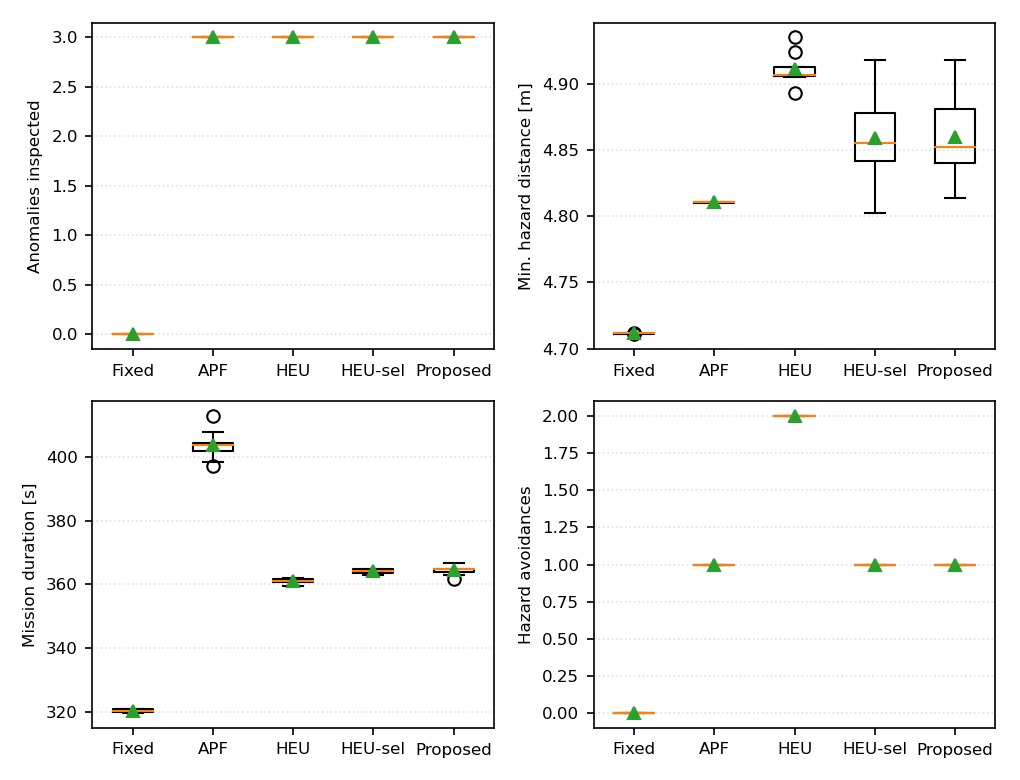
\includegraphics[width=\columnwidth]{box_panel}
\caption{Per-run distributions of the key metrics ($\triangle$ = mean) for the
fixed baseline (E1), the $\eta=0$ ablation (E0), the method (E3), the adverse
scenario (E5), and the potential-field baseline (APF). The fixed baseline never
inspects nor retreats; in the default scenario the affective configurations do so
consistently (tight boxes) with E0 matching E3, and APF matches inspection at a
longer mission duration. The dense adverse scenario (E5) shows a spread in
anomalies inspected---not every run completes all five---consistent with the
density limit reported in Section~\ref{sec:adverse}.}
\label{fig:box}
\end{figure}

\subsection{Detection and Inspection Behavior}
The central result is that the affective layer turns a coverage patrol into an
inspection behavior. The fixed baseline (E1) inspects \emph{no} anomalies: it
follows the round and never deviates ($0.0\pm0.0$). With \textsc{Stay Alert}, the
robot inspects \emph{all three} anomalies in every valid run of the default
scenario, at every setting of $\eta$ including the ablation $\eta=0$ (E0--E4 all
$3.0\pm0.0$; Cliff's $\delta=1$, exact permutation $p=1.1{\times}10^{-5}$ vs.\ E1);
this completeness degrades under high perception noise (Section~\ref{sec:robustness})
and dense clustering (Section~\ref{sec:adverse}), which we quantify honestly. The
artificial-potential-field baseline (APF) also inspects all three ($3.0\pm0.0$),
confirming that a comparably simple reactive scheme can produce the anomaly
response; the difference between the methods lies in efficiency and safety,
discussed below, not in raw inspection count. Fig.~\ref{fig:traj} shows the mechanism: the
affective layer leaves the patrol to reach each anomaly's standoff and returns,
whereas E1 traces the round directly.

\begin{figure}[t]
\centering
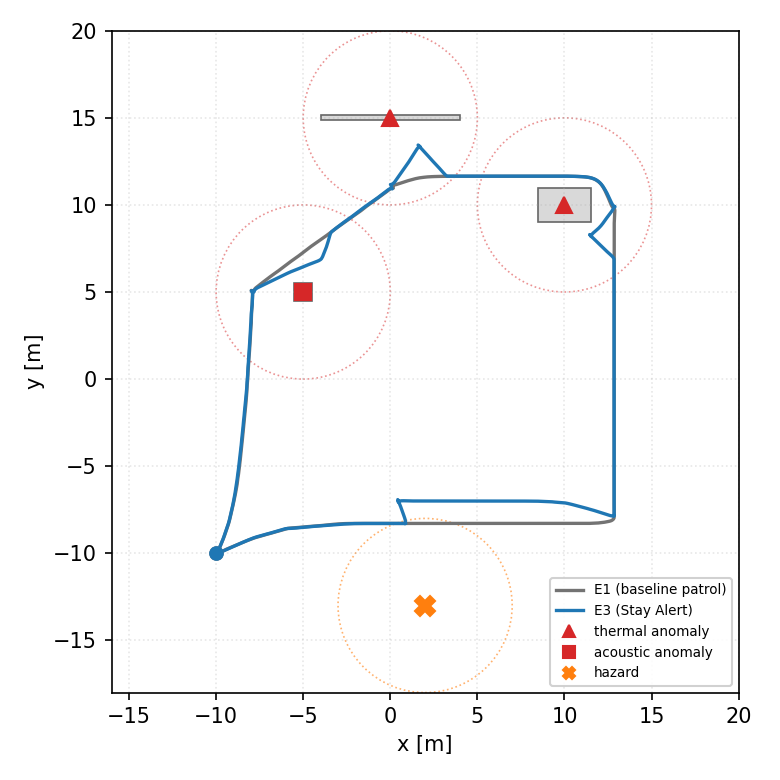
\includegraphics[width=\columnwidth]{traj_overlay}
\caption{Representative trajectories on the default scenario: the baseline
patrol (E1, gray) follows the round directly, whereas the proposed layer
(E3, Stay Alert, blue) deviates to approach the anomalies (thermal $\triangle$,
acoustic $\square$) and skirts the hazard ($\times$) zone. World frame, metres.}
\label{fig:traj}
\end{figure}

\subsection{Isolating the Field from the Act of Deviating}
\label{sec:heu}
%% R2#3: "the baselines fail to separate the affective weighting from a generic
%% same-controller heuristic". Esta subseção é a resposta. Dois contrastes:
%% HEU   = supervisor genérico completo (detecção bruta + seleção por proximidade)
%% HEUsel= UM fator (só o critério de seleção muda); tudo o mais igual ao método.
The comparisons above contrast the reactive layer with baselines that either cannot
deviate (the fixed patrol) or change the controller as well as the supervisor (the
potential-field baseline). Neither isolates the \emph{field} from the act of
deviating at all. We therefore add two configurations that run on the \emph{same}
Nav2/MPPI controller, with the same perception, keep-out, approach poses,
confirmation criterion and return-to-patrol logic:
\begin{itemize}
\item \textbf{HEU}, a generic detect--select--deviate--return supervisor: it is
triggered by \emph{raw detection} (an event inside the sensing radius) rather than by
a threshold on $\Phi$, selects the \emph{nearest} target rather than the most
salient, and arbitrates by the plain rule ``hazard in range $\Rightarrow$ deviate''.
It therefore discards both the saliency weighting and the categorical precedence.
\item \textbf{HEU-sel}, a one-factor variant: identical to the proposed layer
\emph{except} that it selects the nearest rather than the most salient target.
\end{itemize}
Changing the selected target does not alter $\Phi$ at the moment of triggering: the
simulator publishes the intensity of every event in range and the field retains the
maximum, so the threshold crossing is the same in both modes. It does, however, change
which anomaly is committed, and a committed anomaly stops feeding the field; the
contrast is thus one of selection at the decision point \emph{with} a downstream
effect on the time course of $\Phi$, not merely a reordering of service.

Table~\ref{tab:heu} reports the three scenarios. \textbf{Confirmatory (Holm-corrected
within the family declared in advance), \texttt{default} scenario:} HEU-sel is
indistinguishable from the proposed layer on every metric
($p_{\mathrm{Holm}}=1.0000$ throughout; $|\delta|\le0.19$; all bootstrap intervals
contain zero), whereas HEU differs in retreats ($1$ vs.\ $2$,
$p_{\mathrm{Holm}}=0.0034$), investigation time ($35.1$ vs.\ $41.2$~s,
$p_{\mathrm{Holm}}=0.0034$) and mission duration ($p_{\mathrm{Holm}}=0.0052$). The
clearance difference in this scenario does not survive correction
($p_{\mathrm{Holm}}=0.0511$) and amounts to $6$~cm, which we read as operationally
irrelevant and report as such rather than as an advantage.

\textbf{Exploratory, \texttt{conflict} scenario}---where a hazard is co-located with a
\emph{more salient} anomaly, so the two rules disagree by construction---the
difference is large and in the direction the precedence was designed to prevent. HEU
inspects the co-located anomaly (median $4$ of $4$ versus $3$ for the proposed layer)
and pays for it: minimum clearance falls from $4.84$ to $2.23$~m (Cliff's
$\delta=+1.00$, complete separation; bootstrap CI of the difference
$[+2.60,+2.63]$~m; $p<0.0001$), retreats rise from $1$ to $4$ as the supervisor
oscillates, mission duration grows by ${\approx}106$~s, and the time to inspect the
priority target is delayed by ${\approx}105$~s in both modalities
($345.0$ vs.\ $239.9$~s thermal; $387.6$ vs.\ $283.1$~s acoustic). HEU-sel again
matches the proposed layer on every metric.

\textbf{Exploratory, \texttt{adverse} scenario}: all three configurations inspect all
five anomalies; HEU performs one additional retreat and the clearance differences are
of the order of centimetres.

Two conclusions follow, and they point in opposite directions for the two components
of the field. The \emph{selection} rule is inert: replacing saliency by proximity
changed no measured outcome in any of the three scenarios. What is not inert is the
\emph{categorical precedence} carried by the sign of $\Phi$: discarding it, as the
generic supervisor does, trades safety and timeliness for one extra inspection
precisely when a hazard and a salient anomaly coincide. We therefore attribute the
reactive layer's advantage over a generic deviate-and-return heuristic to the
arbitration rule rather than to the saliency weighting, and we note that this is a
narrower claim than the one made in the previous version of this article.

\begin{table*}[t]
\centering
\caption{Proposed layer versus a generic detect--select--deviate--return supervisor
(HEU) and a one-factor selection variant (HEU-sel), all on the same Nav2/MPPI
controller. Medians over valid runs; $n$ per cell in the header. The
\texttt{default} row block is the confirmatory family (Holm-corrected); the
\texttt{conflict} and \texttt{adverse} blocks are exploratory and are reported with
uncorrected $p$.}
\label{tab:heu}
\footnotesize
\setlength{\tabcolsep}{4pt}
\begin{tabular}{llccccc}
\hline
\textbf{Scenario} & \textbf{Metric} & \textbf{Proposed} & \textbf{HEU} &
\textbf{HEU-sel} & \textbf{$\delta$ (vs.\ HEU)} & \textbf{$p$ (vs.\ HEU)}\\
\hline
\texttt{default} & Anomalies inspected        & $3$     & $3$     & $3$     & $+0.00$ & $1.0000^{\dagger}$\\
                 & Hazard retreats            & $1$     & $2$     & $1$     & $-1.00$ & $0.0034^{\dagger}$\\
                 & Min.\ hazard distance [m]  & $4.85$  & $4.91$  & $4.85$  & $-0.73$ & $0.0511^{\dagger}$\\
                 & Investigation time [s]     & $35.1$  & $41.2$  & $35.3$  & $-1.00$ & $0.0034^{\dagger}$\\
\hline
\texttt{conflict} & Anomalies inspected       & $3$     & $4$     & $3$     & $-0.67$ & $0.0160$\\
                 & Hazard retreats            & $1$     & $4$     & $1$     & $-1.00$ & $0.0003$\\
                 & \textbf{Min.\ hazard dist.\ [m]} & $\mathbf{4.84}$ & $\mathbf{2.23}$ & $4.82$ & $+1.00$ & $<\!0.0001$\\
                 & Mission duration [s]       & $363.7$ & $469.7$ & $364.4$ & $-0.89$ & $0.0013$\\
                 & Time to priority target [s]& $239.9$ & $345.0$ & $240.4$ & ---     & ---\\
\hline
\texttt{adverse} & Anomalies inspected        & $5$     & $5$     & $5$     & $-0.10$ & $0.7337$\\
                 & Hazard retreats            & $1$     & $2$     & $1$     & $-1.00$ & $0.0002$\\
                 & Min.\ hazard distance [m]  & $4.88$  & $4.90$  & $4.85$  & $-0.58$ & $0.0288$\\
\hline
\end{tabular}

\vspace{2pt}
\footnotesize $n$: \texttt{default} $10/9/10$, \texttt{conflict} $10/9/10$,
\texttt{adverse} $10/10/10$ (proposed/HEU/HEU-sel).
$^{\dagger}$Holm-corrected within the confirmatory family. Every
proposed-versus-HEU-sel comparison yields $p_{\mathrm{Holm}}=1.0000$ or
$p>0.22$ and is omitted from the last two columns for brevity.
\end{table*}

\subsection{Hazard Response and Safety}
The fixed baseline records zero hazard avoidances, while the affective layer
performs exactly one retreat per encounter ($1.0\pm0.0$). For the hazard placed
\emph{beside} the route (E0--E5), the minimum clearance is small in absolute
terms for both, but the affective layer keeps a slightly \emph{larger} and highly
consistent clearance (E3 $4.86\pm0.03$\,m) than the fixed baseline
($4.71\pm0.00$\,m): the repulsion regulates the approach to a tight band, and
the baseline---now that spawn-failure runs are separated out---passes the
beside-route hazard at a fixed, marginally closer distance. The more informative
test places the hazard \emph{on} a patrol leg (configurations RHM, the method,
and RHB, the fixed baseline). There, the fixed baseline drives straight through,
reaching a minimum clearance of only $0.71\pm0.00$\,m with no retreat and a
minimum time-to-collision of $2.8\pm0.1$\,s, whereas the affective layer produces
a two-timescale response: as soon as the hazard is detected it is projected as a
persistent keepout into the global costmap (so the planner routes around it for the
rest of the mission), and a fast reactive retreat ($1.0\pm0.0$ avoidance event)
handles the immediate proximity; the two together let the robot contour the hazard
at $1.71\pm0.01$\,m ($0$ collisions across valid runs) with a time-to-collision
margin of $5.6\pm0.9$\,s, while still inspecting all three anomalies ($3.0\pm0.0$),
at a time cost of $372\pm1$\,s. The
affective layer thus more than doubles the clearance
($+1.00$\,m; Cliff's $\delta=1$, $p<10^{-4}$) and roughly doubles the
time-to-collision margin ($+2.8$\,s; $p<10^{-4}$) of the fixed patrol on the case
the repulsion is meant to
handle---a hazard blocking the route---demonstrating the affective signal acting
on both the reactive and the deliberative layer (Table~\ref{tab:safety}).

\begin{table}[t]
\centering
\caption{On-route hazard: safety outcomes (mean\,$\pm$\,std over valid runs). RHB
is the fixed baseline (drives straight through); RHM is the method---a reactive
retreat combined with a detection-triggered persistent keepout that the planner
routes around. Valid $n$: RHB $10$, RHM $9$.}
\label{tab:safety}
\footnotesize
\begin{tabular}{lcc}
\hline
\textbf{Metric} & \textbf{RHB (baseline)} & \textbf{RHM (method)}\\
\hline
Anomalies inspected        & $0.0\pm0.0$   & $3.0\pm0.0$\\
Hazard retreats            & $0.0\pm0.0$   & $1.0\pm0.0$\\
Collisions                 & $0.0\pm0.0$   & $0.0\pm0.0$\\
Min.\ hazard distance [m]  & $0.71\pm0.00$ & $1.71\pm0.01$\\
Min.\ time-to-collision [s]& $2.8\pm0.1$   & $5.6\pm0.9$\\
Time below clearance [s]   & $14.4\pm0.0$  & $9.2\pm0.1$\\
Mission duration [s]       & $320\pm1$     & $372\pm1$\\
\hline
\end{tabular}
\end{table}

To attribute this safety gain to its two mechanisms, we ablate them
(Table~\ref{tab:ablation}). With the \emph{keepout alone} (KOa, reactive retreat
disabled) the planner still routes around the hazard and inspects all three
anomalies at the same $1.71$\,m clearance, slightly faster than the full method
($352$ vs.\ $372$\,s). With the \emph{reactive retreat alone} (KOb, keepout
disabled) the robot cannot clear the on-route hazard: it oscillates
($29.6\pm3.9$ retreats), inspects almost nothing ($0.2\pm0.4$), and times out
($627\pm6$\,s). %% R3#2: "A fairer reference for the safety claim is the fixed patrol plus the same
%% detection-triggered keepout, with no reactive layer at all." KOF e exatamente isso.
These two ablations still carry the reactive layer. Reviewer comment R3.2 asks for the
fairer reference: a \emph{fixed patrol carrying the same detection-triggered keep-out
and no reactive layer at all}. We therefore add configuration KOF (reactive layer
disabled, keep-out enabled). KOF reaches a median minimum clearance of $1.73$~m
against $1.71$~m for the keep-out-only ablation KOa---a difference of $2$~cm that is
not distinguishable ($p_{\mathrm{Holm}}=0.42$)---and spends $9.0$~s below the $2$~m
band against $9.3$~s. \textbf{We therefore attribute the safety benefit on an on-route
hazard to the detection-triggered keep-out, not to the reactive weighting}, and we
state this in the abstract and the conclusion rather than leaving the comparison
against a hazard-blind baseline to carry the claim.

What the reactive layer contributes over KOF is the inspection behavior itself, and
only that: KOF inspects $0$ of the $3$ anomalies in every run---by construction, since
with no reactive layer no investigation is ever triggered---against $3$ of $3$ for
KOa ($p_{\mathrm{Holm}}=0.0027$), and it completes the mission $31$~s faster
($320.9$ vs.\ $352.1$~s, $p_{\mathrm{Holm}}=0.0027$) precisely because it never
detours. The honest reading of the pair KOF/KOa is therefore a decomposition rather
than a victory: the keep-out buys the clearance, the reactive layer buys the
inspections, and they are separable.

The deliberative keepout is therefore the mechanism that resolves
an on-route hazard; the reactive retreat adds \emph{no} measurable benefit for this
\emph{static} hazard (KOa matches RHM and is slightly faster). We do not claim the
retreat helps here---its value instead appears when a hazard \emph{emerges} during
an investigation, which we quantify next (Section~\ref{sec:emerging}).

\begin{table}[t]
\centering
\caption{Keepout/retreat ablation on the on-route hazard (mean\,$\pm$\,std over
valid runs; $n=9$ for RHM, $10$ for KOa, $9$ for KOb). RHM is the full method
(retreat $+$ keepout); KOa is keepout-only (retreat disabled); KOb is retreat-only
(keepout disabled).}
\label{tab:ablation}
\footnotesize
\setlength{\tabcolsep}{5pt}
\begin{tabular}{lccc}
\hline
\textbf{Metric} & \textbf{RHM} & \textbf{KOa} & \textbf{KOb}\\
 & \textbf{(re.+ke.)} & \textbf{(keep.)} & \textbf{(retr.)}\\
\hline
Anomalies inspected        & $3.0\pm0.0$   & $3.0\pm0.0$   & $0.2\pm0.4$\\
Hazard retreats            & $1.0\pm0.0$   & $0.0\pm0.0$   & $29.6\pm3.9$\\
Collisions                 & $0.0\pm0.0$   & $0.0\pm0.0$   & $0.0\pm0.0$\\
Min.\ hazard distance [m]  & $1.71\pm0.01$ & $1.71\pm0.01$ & $4.29\pm0.08$\\
Min.\ time-to-collision [s]& $5.6\pm0.9$   & $5.8\pm0.1$   & $8.7\pm0.2$\\
Mission duration [s]       & $372\pm1$     & $352\pm1$     & $627\pm6$\\
\hline
\end{tabular}
\end{table}

\subsection{The Retreat's Value under an Emerging Hazard}
\label{sec:emerging}
The ablation above shows that, for a \emph{static} on-route hazard, the
deliberative keepout alone (KOa) matches the full method and the reactive retreat
adds no measurable benefit. The retreat is designed, however, for a hazard that
\emph{emerges} while the robot is already committed to an inspection---the case the
preemption of Algorithm~\ref{alg:stayalert} was built for and that the static
scenarios cannot exercise. We test this directly (configurations DHa, DHb): a
hazard co-located with an anomaly stays inactive---published to neither the
reactive channel nor the deliberative keepout---until the robot, already
investigating, closes to $3$~m, at which point the environment activates it (the
activation instant and the first publication to each channel are logged per run).
The clearance and radial time-to-collision values below are \emph{whole-mission}
minima relative to the hazard's location, including the pre-activation period: the
collector does not reset these metrics upon activation. These results therefore
compare overall mission-level margins in the emerging-hazard scenario and do not
estimate a separate post-activation TTC effect. The audit's preserved simulation
time does let us localize the \emph{distance} minimum: it is reached after
activation in all $18$ valid dynamic runs. We do \emph{not} extend this to the TTC
minimum---which, being a ratio involving radial speed, can already carry a
pre-activation value (in one run the final TTC minimum is recorded just before
activation)---so the TTC difference is reported strictly as a whole-mission margin. With the
reactive retreat enabled (DHa) the preemption fires in \emph{every valid run}
($8/8$ deferred investigations) and the robot backs off, keeping a minimum
clearance of $2.55\pm0.15$\,m and a radial time-to-collision of $5.23\pm0.45$\,s.
With the retreat disabled (DHb, keepout only) the robot instead proceeds to the
inspection standoff, closing to $2.22\pm0.01$\,m ($4.72\pm0.21$\,s). The reactive
retreat therefore buys $+0.33$\,m of clearance ($95\%$ CI $[+0.23,+0.42]$, Cliff's
$\delta=1$, $p=4.6{\times}10^{-5}$) and $+0.51$\,s of time-to-collision margin
($[+0.20,+0.84]$, $\delta=0.85$, $p=1.0{\times}10^{-3}$) against an emerging
hazard. This margin is a deliberate trade, not a free gain: DHa runs about
$9.4$~s longer ($348$ vs.\ $338$~s) and $1.6$~m farther, and \emph{defers} the
now-hazardous inspection (DHa inspects the target in no run; DHb in every run),
buying a larger safety margin at that encounter at the price of a completed
inspection. Neither configuration enters the contact region, and neither spends
any time below the $2$~m clearance threshold, so the effect is a difference in
\emph{margin}, not in observed contacts. We also distinguish the preemption
firing from a cleanly completed retreat: in $3$ of the $8$ valid DHa runs the
retreat's navigation goal is itself aborted, yet each episode still ends as a
successful avoid---the field decays below threshold once the hazard is handed to
the keepout (\emph{safe} exit)---and the clearance we report is the
\emph{true-position} minimum from the metrics collector, not an assumed arrival at
the retreat pose (those three runs in fact hold $2.70$~m). The retreat's
contribution is thus a \emph{transient} safety margin when a hazard appears
mid-investigation---a benefit the static on-route ablation, by construction,
cannot reveal.

\subsection{Safety Precedence under Conflict}
\label{sec:conflict}
The preceding scenarios separate attraction and repulsion in space, so the field
never has to arbitrate between an anomaly and a hazard at the same location. The
conflict scenario (CONF) forces exactly that decision: a \emph{strong} acoustic
anomaly ($|w\,I_e|=1.14$) is co-located with a \emph{weaker} hazard
($|w\,I_e|=1.05$) at $(2,-13)$, so a magnitude-only selection rule---which keeps
the more salient signal---would prefer to inspect the anomaly and never trigger
a retreat. The precedence rule of Eq.~\eqref{eq:phi-update} instead resolves any
above-threshold hazard first, independently of a concurrent, stronger attraction.
This is a categorical \emph{selection} property, not an average effect, so we
report it as an outcome frequency rather than a mean comparison. Across all ten runs of CONF
(all valid), the behavior was identical in every run: \textsc{Avoid} was
triggered ($10/10$ runs, $1.0\pm0.0$ retreats) and the co-located strong anomaly
was \emph{never} inspected, so the robot inspected only the three off-conflict
anomalies ($3.0\pm0.0$; the fourth event is the co-located pair). The robot kept a
minimum hazard clearance of $4.84\pm0.02$\,m and a minimum time-to-collision of
$17.3\pm1.6$\,s, with \emph{zero} collisions across all runs, at a mission duration
($364\pm2$\,s) indistinguishable from the default scenario. The affective
field therefore enforces a \emph{hazard-first selection priority} by construction,
confirmed empirically in the one case designed to break a magnitude-only
interpretation. This is a deliberate design choice---the priority is \emph{hard},
so a hazard barely above threshold (a potential false positive) suppresses even a
strongly salient genuine anomaly---and we accept the resulting risk of
over-conservatism near the threshold. We distinguish this \emph{logical} priority
from a physical safety guarantee: it holds under explicit conditions (an available
retreat pose, and outside the post-retreat refractory window), and the static CONF
scenario does not exercise cases such as a second hazard appearing during the
refractory; what we report as a safety \emph{outcome} is the observed clearance and
the absence of contact-region entries, not an invariance guarantee.

\subsection{The Cost of the Precedence, and Its Sensitivity}
\label{sec:precedence-cost}
%% R2#6: "A hazard barely above threshold suppresses even a strongly salient genuine
%% anomaly, and the authors acknowledge the resulting over-conservatism risk. A
%% sensitivity analysis around the hazard threshold, or a scenario with a marginal
%% hazard and a high-value inspection target, would strengthen the claim that the
%% precedence is not merely correct-by-construction but also operationally sensible."
%% Fazemos as duas coisas. Exploratorio.
The preceding subsection accepts a risk of over-conservatism near the threshold
without measuring it. We now measure it, and separately probe whether the threshold
that governs the precedence is well placed. Both analyses are exploratory.

\paragraph*{A marginally eligible hazard costs one inspection, deterministically}
The hazard channel has memory: an observation raises $h$, and $h$ then decays by
$\lambda$ per period until it falls below $\varepsilon$. Because the modality
threshold is applied to the raw perceived intensity, the \emph{weakest} eligible
hazard already yields $h=|w_{\mathcal{H}}|\,\theta_{\mathcal{H}}$, which here equals
the supervisor's entry threshold; a retreat therefore fires once, at the peak. After
a single decay step, however, $h$ is below the entry threshold while still above
$\varepsilon$---so the hazard keeps \emph{governing} the field, and thus keeps
suppressing any attraction, without triggering any further retreat. We built
configuration CM to exercise exactly this band: a hazard of minimal eligible
intensity beside the first patrol leg, which the robot observes and then leaves
behind, together with a legitimate acoustic anomaly of intensity $0.95$---the most
salient event in the scenario---placed $4.3$~m from the hazard, well outside it.

The result is deterministic across all ten runs. The suppression window lasts
$69.5$~s (range $67.3$--$72.4$), exactly one retreat fires, and the salient anomaly
is \emph{never} inspected: $0/10$ runs, so the robot ends every mission having
inspected $3$ of the $4$ anomalies, and the one it forfeits is the strongest. The
priority-target metric records the same outcome from the other side: the acoustic
priority target is censored at the $400$~s horizon in $10/10$ runs. The categorical
precedence therefore does not merely risk over-conservatism---in this configuration
it costs one inspection in every run, and the cost is incurred while the robot is in
no danger, since the hazard is by then too weak to warrant retreating from.

We emphasise one reading that the numbers do not support. CM and the full conflict
scenario both end with three anomalies inspected, but the two threes are not
comparable: in CONF the forfeited anomaly is co-located with the hazard and
\emph{should} be refused, whereas in CM it is a legitimate target $4.3$~m away. The
same count is correct behavior in one scenario and a failure in the other.

\paragraph*{The threshold governing the precedence is well placed, and raising it
costs clearance} Varying the supervisor's entry threshold does not test the
precedence, because what governs suppression is the \emph{modality eligibility}
threshold $\theta_{\mathcal{H}}$ applied before weighting. We sweep that threshold
over $\{0.20,0.30,0.40\}$ in the conflict scenario, with $0.30$ the value used
throughout. Lowering it to $0.20$ changes nothing measurable (clearance $4.85$ vs.\
$4.83$~m, $p=0.39$; identical inspections and retreats). Raising it to $0.40$
\emph{degrades} safety: the minimum clearance falls to $3.78$~m (Cliff's
$\delta=+1.00$, bootstrap CI of the difference $[+0.99,+1.10]$~m, $p<0.0001$) and the
mission lengthens by $9.1$~s, because a higher eligibility threshold means the hazard
is recognised later and therefore closer. The sweep thus yields a conclusion rather
than a range: the operating point is at a plateau on one side and a cliff on the
other, and the clearance reported elsewhere in this article is not an artifact of a
conveniently chosen threshold.

\paragraph*{Hysteresis: width is immaterial, position is not}
%% R3#3 pede os valores de histerese e limiar como sensibilidade. Os tres pares
%% separam POSICAO de LARGURA -- um par que mude as duas coisas nao permitiria
%% atribuir o efeito.
We compare three entry/exit pairs chosen so that position and width vary
independently: the reference $(0.45,0.25)$ of width $0.20$; a narrower band
$(0.45,0.35)$ of width $0.10$ at the same entry point; and a shifted band
$(0.55,0.35)$ of the same width $0.20$. Halving the width changes nothing: route
deviations, inspections, mission duration and investigation time are all
indistinguishable from the reference ($p\ge0.60$). Shifting the entry point doubles
the counted route deviations ($4\rightarrow8$, $\delta=-1.00$, $p=0.0003$) and
shortens the mean investigation episode ($35.1\rightarrow26.6$~s, $p=0.0003$), while
leaving the inspections unchanged at $3$ of $3$: with a higher entry threshold the
robot lingers longer in the aroused-but-uncommitted band and commits closer to the
target. The behavior of interest is therefore robust to the hysteresis width, and the
\texttt{route deviations} metric should be read as sensitive to the \emph{position}
of the entry threshold rather than as a scenario-intrinsic count.

\subsection{Cost of the Inspection Behavior}
The added behavior is inexpensive: the mission duration of E3 ($364\pm1$\,s) is a
modest increase over the fixed baseline ($320\pm1$\,s) for the inspection
detours ($+6.2$\,m travelled). Framed as a utility trade-off, each additional
anomaly inspected costs about $2$\,m of extra travel ($+6.2$\,m for three) and
$15$\,s of mission time ($+44$\,s for three)---a favorable exchange given that
the fixed baseline inspects \emph{none}.

%% R3#3 pede a comparacao com o APF consolidada numa tabela unica, com intervalos,
%% e a declaracao do procedimento e do ESFORCO de ajuste. Tambem corrigimos aqui a
%% afirmacao da versao anterior de que o baseline de mesmo controlador ficava como
%% trabalho futuro: ele agora existe (Secao~\ref{sec:heu}).
Table~\ref{tab:apf} consolidates the comparison against the potential-field
baseline, which the previous version of this article reported across several tables.
The proposed layer completes the same three inspections faster ($364$ vs.\
$404\pm5$\,s). We are explicit about what this does \emph{not} isolate: the APF
baseline replaces the reactive supervisor \emph{and} the controller---it commands
velocities directly instead of issuing Nav2/MPPI goals---so the difference confounds
the supervisor with the controller. On tuning effort we are equally explicit: the APF
gains were set by manual sweep until the baseline completed the default scenario
without local-minimum stalls, and its approach parameters differ from ours (standoff
$1.8$~m and a $30$~s investigation budget, against $2$~m and $40$~s;
Table~\ref{tab:hyper}). We did not invest comparable effort in tuning the baseline's
thresholds to those of the proposed layer, and the time advantage should be read with
that asymmetry in mind. The comparison that \emph{does} isolate the supervisor, on a
shared controller and shared parameters, is the heuristic of Section~\ref{sec:heu};
the earlier version of this article left that baseline as future work and it is now
part of the study.

\begin{table}[t]
\centering
\caption{Consolidated comparison against the potential-field baseline (default
scenario, valid runs; $n=10$ proposed, $n=9$ APF). Mean\,$\pm$\,std, with the $95\%$
bootstrap interval of the difference. The two configurations differ in both
supervisor and controller, so the difference is not attributable to the reactive
layer alone.}
\label{tab:apf}
\footnotesize
\setlength{\tabcolsep}{4pt}
\begin{tabular}{lccc}
\hline
\textbf{Metric} & \textbf{Proposed (E3)} & \textbf{APF} & \textbf{$95\%$ CI of diff.}\\
\hline
Anomalies inspected        & $3.0\pm0.0$   & $3.0\pm0.0$   & $[+0.00,+0.00]$\\
Mission duration [s]       & $364\pm1$     & $404\pm5$     & $[-43.1,-36.8]$\\
Distance travelled [m]     & $86.6\pm0.2$  & $88.9\pm1.1$  & $[-3.1,-1.6]$\\
Min.\ hazard distance [m]  & $4.86\pm0.03$ & $4.79\pm0.06$ & $[+0.03,+0.11]$\\
Time to priority target [s]& $240.8$       & $269.7$       & $[-34.2,-23.1]$\\
\hline
\end{tabular}
\end{table}

\subsection{Adverse Scenario}
\label{sec:adverse}
In the event-dense scenario (E5) the robot arbitrates between clustered events by
the precedence rule of Eq.~\eqref{eq:phi-update}, inspecting on average
$4.9\pm0.3$ of the five anomalies with correspondingly more deviations
($9.4\pm0.8$) and a longer mission ($397\pm4$\,s). Full inspection of all five
succeeds in $9$ of $10$ runs ($95\%$ Wilson interval $[0.60,0.98]$). The
per-episode audit trail (Section~\ref{sec:setup}) shows the cause precisely: all
five targets are \emph{started} in every run, and the incompleteness is a
navigation failure, not a failure to revisit. Three runs recorded a reactive
navigation failure; two of them subsequently \emph{started an additional
investigation} and completed all five targets, while the remaining run ended with
four credited inspections and \emph{no further recorded attempt} on the failed
target. The two additional investigations are reported as an observation of the
episodes, not as a demonstrated retry policy: the \texttt{failed} branch marks the
target as failed but does not remove it from the committed set, so a later start is
possible but not guaranteed by an explicit recovery rule. This density limit---the
reactive navigation occasionally failing on a tightly clustered target---is measured
honestly here rather than assumed away, with no contact-region entries observed
(zero collisions). We do not claim general scaling from a single adverse
configuration, and broader density and geometry sweeps remain future work.

%% R3#1 (reposicionamento editorial): a subseção 'Value-Function Stability' e a
%% Fig. do resíduo foram movidas para o Apêndice~\ref{app:update} junto com a
%% formulação. Elas atestam que o update é estável, não que ele governe
%% comportamento -- manter no corpo dava-lhes um peso que o resultado não sustenta.

\subsection{Robustness to Perception Noise}
\label{sec:robustness}
Because the event abstraction supplies modality, intensity, and position without
uncertainty, we probe the method's sensitivity to this idealization by injecting
zero-mean Gaussian noise on the perceived event position and intensity at each
sensing tick. Under moderate noise (position $\sigma=0.3$\,m, intensity
$\sigma=0.05$; configuration N1) the method is unaffected: it inspects all three
anomalies in every valid run ($3.0\pm0.0$), with the hazard response preserved and
no collisions. Under high noise ($\sigma=0.6$\,m, $\sigma=0.10$; N2), inspection
completeness degrades to $4/9$ full inspections, and the run logs let us attribute
the cause precisely: all three anomalies are still \emph{detected} in every run, but
the noisy position estimate steers the robot to a point from which the evaluator
cannot confirm arrival at the \emph{true} anomaly, so $6$ of the $27$ committed
inspections (across the $9$ valid runs) are \emph{confirmation rejections}---not
navigation timeouts or aborts, of which the CSVs record none. Full inspection
therefore succeeds in $4$ of $9$ valid runs ($2.3\pm0.7$ anomalies; $95\%$ Wilson
interval $[0.19,0.73]$ for the per-mission completion rate). No contact-region
entries were observed, and the hazard retreat was preserved ($1.7\pm0.5$;
Table~\ref{tab:noise}); the mean minimum hazard clearance in fact \emph{increased}
from $4.86\pm0.03$\,m in E3 to $5.29\pm0.20$\,m in N2. These results describe the
observed trade-off under the tested noise levels---inspection completeness falls
(through the confirmation step) while no contacts are observed and the measured
clearance grows---and do not establish a general safety guarantee. We report per-mission completion with its Wilson
interval rather than treating the three anomalies of a run as independent trials.

\begin{table}[t]
\centering
\caption{Robustness to perception noise (method, mean\,$\pm$\,std). E3 is
noiseless; N1 and N2 add moderate and high zero-mean Gaussian noise on event
position ($\sigma_p$) and intensity ($\sigma_i$). ``Full-inspection rate'' is the
per-mission fraction of runs inspecting all three anomalies (with the confirmed
arrival of Section~\ref{sec:results}); safety (collisions, clearance) is
maintained across all noise levels. Valid $n$: E3 $10$, N1 $10$, N2 $9$.}
\label{tab:noise}
\footnotesize
\begin{tabular}{lccc}
\hline
\textbf{Metric} & \textbf{E3 (none)} &
\textbf{N1 ($\sigma_p{=}0.3$)} & \textbf{N2 ($\sigma_p{=}0.6$)}\\
\hline
Anomalies inspected       & $3.0\pm0.0$  & $3.0\pm0.0$  & $2.3\pm0.7$\\
Full-inspection rate      & $10/10$      & $10/10$      & $4/9$\\
Hazard retreats           & $1.0\pm0.0$  & $1.1\pm0.3$  & $1.7\pm0.5$\\
Collisions                & $0.0\pm0.0$  & $0.0\pm0.0$  & $0.0\pm0.0$\\
Min.\ hazard distance [m] & $4.86\pm0.03$& $5.01\pm0.11$& $5.29\pm0.20$\\
Mission duration [s]      & $364\pm1$    & $367\pm5$    & $374\pm8$\\
\hline
\end{tabular}
\end{table}

\paragraph*{Is the degradation a property of the method or of the confirmation
criterion?}
%% R2#5: "if the confirmation distance is 3.3 m and the noisy position estimate
%% steers the robot away from the true anomaly, is the reported degradation a
%% property of the method or of the confirmation criterion? A sensitivity analysis
%% over the confirmation distance would help disentangle these."
%% O criterio e uma funcao de PONTUACAO pura: nao realimenta o comportamento (a
%% supressao de re-atracao depende de 'committed', marcado no inicio do episodio, e
%% a nao-confirmacao nao o libera). Logo a varredura e RETROSPECTIVA, sobre as
%% MESMAS trajetorias, sem executar nada de novo.
An inspection is credited only if the robot is within a confirmation distance of the
\emph{true} event position when the episode closes; we use $3.3$~m. This criterion
scores the outcome and does not feed back into the controller---the suppression of
re-attraction keys on the target being committed at the \emph{start} of an episode,
and a non-confirmation does not release it---so the same recorded trajectories can be
re-scored under other thresholds without executing anything new. We do so
retrospectively, and label it as such.

Re-scoring reproduces the published figure exactly at $3.3$~m ($4/9$ full inspections
under high noise), which validates the procedure. It also shows the reported
completeness to be strongly criterion-dependent: at $2.8$~m the high-noise rate falls
to $2/9$, and at $4.0$~m it recovers to $9/9$. The robot did approach the anomalies;
under high noise it stopped $2.9$--$3.6$~m away because the perturbed position
estimate displaced the inspection pose, and the $3.3$~m criterion then refused those
approaches. That is only half the answer, however, because the physical approach also
degrades: the distance to the true target at episode close rises from $2.23$~m
(median, range $2.21$--$2.24$) with clean perception to $2.87$~m (range
$1.83$--$3.56$) under high noise. Both effects are present and we report them
together; the defensible statement is that \emph{the completeness figure is sensitive
to the confirmation criterion and the approach quality genuinely degrades}, not that
the degradation is an artifact. We note the measured quantity is the distance at
episode close, not the minimum over the approach, which is not instrumented per run.

\paragraph*{Does the discontinuity at $d=R$ affect the state machine?}
%% R2#8: "the profile still produces an intensity of Ie/2 at the boundary and zero
%% immediately beyond, which is a discontinuity in the reported signal. A brief
%% statement of whether this discontinuity has any measurable effect on the FSM
%% transitions would be useful."
%% Uma contagem global de transicoes nao identificaria o efeito da fronteira, e uma
%% trajetoria tangente poderia so tocá-la. A ronda real cruza d=R nos dois sentidos
%% varias vezes por run, entao medimos sobre os logs existentes.
The intensity profile is $I_e/2$ at $d=R$ and zero immediately beyond, a step in the
reported signal. The patrol crosses this boundary in both directions several times
per run, so we measure its effect on the existing logs rather than constructing a
dedicated trajectory---a tangential path risks touching the boundary without crossing
it. Taking a gap in the field trace as time spent outside every sensing radius, the
first sample after a gap is an inward crossing and the last before it an outward one.
Across the default scenario we observe $30$ inward and $30$ outward crossings in ten
runs, with a median jump at entry of $0.436$ (maximum $0.686$), consistent with the
$|w\,I_e/2|$ predicted by the profile: the discontinuity is real and of the expected
size. Only $10$ of those $30$ inward crossings are followed by a state transition
within $2$~s, so the step does not reliably drive the machine. The shortest interval
between consecutive transitions is $9.8$~s in the default scenario and $7.0$--$9.6$~s
in the noise and conflict scenarios, with no sign of boundary chattering. In the
dense scenario the shortest interval is $0.2$~s, and inspection of those cases shows
they are not threshold oscillation: they are either back-to-back servicing of a
cluster---one anomaly credited and the next, already well inside range at
$\Phi\approx0.5$, committed immediately---or an episode ended at once by a transient
Nav2 goal abort. Neither arises from the boundary.

\subsection{Threats to Validity}
The evaluation is in simulation; field behavior may differ. The
sensing-and-perception chain is abstracted as events, so the inspection rate
measures the \emph{navigation-and-decision} response, not perception accuracy;
we probe sensitivity to this abstraction with the perception-noise sweep
(Section~\ref{sec:robustness}), which also exposes the method's limits: inspection
completeness degrades under high perception noise ($4/9$) and dense clustering
($9/10$) (measured, not assumed), while no contact-region entries were observed in
any scenario. The safety metrics are
proxies computed from the \emph{true} hazard position and should be read as such:
``collisions'' counts entries into a simulated contact region (centre-to-centre
distance below $0.5$~m), not readings of a physical contact sensor, and
``time-to-collision'' is a radial-closing proxy ($d/\dot d$ to the nearest hazard),
not the trajectory-intersection time with a finite hazard region; zero collisions
in a group bounds but does not eliminate risk (the \emph{exact} one-sided $95\%$
binomial bound on the failure probability for zero observed failures,
$1-0.05^{1/n}$, is $\approx26\%$ for a $10$-run group, $\approx28\%$ for a
$9$-run group, and $\approx31\%$ for the $8$-run DHa group; this risk bound is
distinct from the Wilson-score intervals used for the descriptive success rates).
%% R3-m2: "Please give the per-configuration counts in the main text next to the
%% headline numbers, since results such as 4/9 depend on them, and note whether the
%% exclusion could favor any configuration." A segunda parte e a desconfortavel.
A fraction of runs ($6$ of $160$ in the earlier battery, $3$ of $130$ in the new
one) remained immobile (travelled distance $\approx0$); these are reported
separately as a startup-reliability outcome and excluded from the behavioral
statistics. The valid counts are $n=10$ for every configuration except APF, KOb, N2
and RHM ($n=9$), DHa ($n=8$), and the two new heuristic blocks in the
\texttt{default} and \texttt{conflict} scenarios ($n=9$); every rate in this article
is reported against its own denominator, which is why the high-noise completeness
reads $4/9$ and the dense-clustering completeness $9/10$.

Whether the exclusion can favor a configuration deserves a direct answer rather than
an assumption of independence, and the answer differs by metric. All excluded runs
inspected zero anomalies, so removing them \emph{raises} every completeness figure;
for the pair most affected it raises the proposed layer and the APF baseline by the
same amount ($2.7\rightarrow3.0$ anomalies each), leaving their difference unchanged
but making both absolute figures conditional on successful initialization. For
safety the adjustment runs the other way: a run in which the robot never moved
trivially records zero contact-region entries, so including such runs would inflate
the evidence for contact-free navigation, and they are therefore excluded from the
safety statistics as well. We do not claim that start-up failure is independent of
configuration---the exclusions are not uniformly distributed across blocks---only
that the direction of each adjustment is stated and that both views are reported. Event identity and inspection pose are published on
separate topics within the same sensing tick rather than as one timestamped
message; for the single-salient-target dynamics evaluated here they refer to the
same observation, but guaranteeing this under rapid target switching is left as an
implementation refinement. Localization is idealized---the
map$\rightarrow$odom transform is held fixed---so localization drift is not modeled
(Section~\ref{sec:setup-repro}). The value function is tabular, and the
value-update formulation is a design note (Appendix~\ref{app:update}) rather than
the mechanism controlling the robot here. These
choices are documented for reproducibility (Section~\ref{sec:setup-repro}).

%% R2-Q3: "the limitations section is candid, but several acknowledged gaps are
%% stated rather than probed". Tres delas passaram a ser medidas nesta versao.
Three gaps that earlier versions of this article acknowledged without probing are now
measured, and we point to the measurements rather than repeating the acknowledgement.
The risk of over-conservatism near the hazard threshold is quantified in
Section~\ref{sec:precedence-cost}, where a marginally eligible hazard is shown to
cost one inspection in every run; the sensitivity of the reported completeness to the
confirmation criterion is quantified by re-scoring the same trajectories at other
thresholds; and the claim that the reactive layer outperforms a generic
deviate-and-return behavior is now tested directly against such a behavior on the
same controller (Section~\ref{sec:heu}), with the result that the saliency weighting
is inert and only the arbitration survives. The gaps that remain stated rather than
probed are those requiring a different perception model: false positives and
negatives, event persistence, and localization drift.

\paragraph*{Provenance of the field signal} For auditability we note that the value
of $\Phi$ written into the value update is sampled in the odometry callback, whereas
the value published to the reactive supervisor is sampled by a $1$~Hz timer. Both
read the same field object, so they differ only in sampling instant; this does not
affect the executed behavior, which is driven by the published signal, but it means
the two series in the released logs are not sample-aligned.

\section{Conclusion}
\label{sec:conclusion}
%% R3#1/R2#1: a conclusão espelha o abstract reposicionado -- nada de Bellman/RL
%% como contribuição. R3-m1: a qualificação de escopo (percepção oráculo,
%% localização fixa) aparece aqui, não só na §limitações. R2#4: o bound binomial
%% está na MESMA frase da ausência de contatos.
We presented a two-layer navigation architecture for substation inspection: a
deliberative active-sensing patrol carries the sensors to where events may occur,
and a reactive layer produces a threshold-triggered approach impulse toward
anomalies and a retreat impulse from hazards, from an attraction/repulsion field
$\Phi$ derived from sensory saliency and arbitrated by a categorical safety
precedence. The architecture runs on a mature, reproducible stack (ROS~2 +
Nav2/MPPI + Gazebo Fortress).

The evaluation narrows what may be credited to the reactive layer, and we state the
three attributions plainly. First, on a hazard placed on the patrol route, a
\emph{hazard-blind patrol carrying the same detection-triggered keep-out} reaches a
minimum clearance indistinguishable from the full method ($1.73$ vs.\ $1.71$~m;
$p_{\mathrm{Holm}}=0.42$), so the safety benefit is attributable to the deliberative
keep-out rather than to the reactive weighting; the reactive layer's contribution
there is the inspections themselves ($3$ vs.\ $0$ of $3$) at a cost of $31$~s.
Second, the \emph{selection} rule is inert: a variant differing only in selecting the
nearest instead of the most salient target reproduced the method in every scenario
and every metric. What is not inert is the categorical precedence---a generic
detect--select--deviate--return heuristic on the same Nav2/MPPI controller, driven by
raw detection, inspects the anomaly co-located with a hazard and halves the minimum
clearance ($4.84$ vs.\ $2.23$~m, Cliff's $\delta=+1.00$) while delaying the priority
inspection by ${\approx}105$~s. Third, that precedence carries a measured cost: a
marginally eligible hazard suppresses attraction for ${\approx}70$~s and forfeits one
of four inspections in $10/10$ runs. Taken together, the arbitration rule---not the
saliency weighting---is what distinguishes this layer from a generic deviate-and-return
heuristic, and it trades completeness for clearance in a way that is now quantified in
both directions.

Inspection completeness is reported as the rate of runs inspecting \emph{all}
anomalies: $10/10$ with clean perception, $4/9$ under high perception noise and
$9/10$ under dense clustering. A retrospective re-scoring shows this rate is strongly
sensitive to the confirmation criterion (at a $4.0$~m threshold the high-noise rate
recovers to $9/9$), while the physical closing distance does degrade
($2.23 \rightarrow 2.87$~m median), so both effects are present. No entry into the
$0.5$~m contact region was observed in any configuration, but with $8$--$10$ valid
runs per group the exact one-sided $95\%$ bound on the per-run probability of such an
entry remains $25.9$--$31.2\%$; and on the on-route hazard the method transits
\emph{within} the $2$~m advisory clearance band it reports, for ${\approx}9$~s per
run. These are the limits of the safety evidence, not a safety guarantee.

\paragraph*{Scope} The evaluation is in simulation. Perception is abstracted to
oracle events rather than raw sensor streams, and the localization transform is held
fixed, so the results characterize the \emph{decision logic} of the architecture and
should not be read as validating a deployable autonomous inspection system. The
$0.5$~m contact region and $2$~m clearance band are operationally defined
centre-to-centre distances used as measurement proxies---with a $0.25$~m robot
radius---not physical contact sensing and not regulatory electrical clearances.

\paragraph*{Limitations} Localization error, event persistence, false positives and
negatives, and map geometry are left unmodelled. The adverse scenario is a single
dense configuration and the noise sweep covers two levels, so neither supports a
general scaling claim. The value table is tabular and, as Appendix~\ref{app:update}
records, does not select the executed actions; we therefore make no convergence or
policy-invariance claim for the augmented update.

\paragraph*{Future work} The inert selection rule and the quantified cost of the
precedence both point the same way: the arbitration, not the weighting, is where
further work belongs. A policy that \emph{learns} when to defer to the hazard channel
instead of always deferring would address the over-conservatism we measured, and the
value formulation in Appendix~\ref{app:update} is the natural substrate for it---but
it requires an exploration policy, an action-to-velocity mapping and a comparison
against ordinary tabular Q-learning, which is beyond this study. We also plan
hardware-in-the-loop validation on the quadruped GO2~PRO platform and a field trial
at the Axia substation (Araraquara, Brazil), with real thermal, acoustic and visual
perception driving the event layer.


\appendices
\section{Event Layout}
\label{app:params}
Table~\ref{tab:events} lists the simulated events for all six scenarios (positions
in world metres; $I_e$ is the base intensity). The patrol waypoints are
$(13,-8)$, $(13,10)$, $(0,11)$, $(-8,5)$, $(-10,-10)$. The remaining method and
simulation parameters are given in Table~\ref{tab:hyper}.

\begin{table}[h]
\centering
\caption{Simulated events for all six scenarios (positions in world metres;
$I_e$ is the base intensity). In \emph{dyn-hazard} the repulsive event is
co-located with the anomaly and \emph{activates}---starts being published to
both the reactive and keepout channels---only when the robot reaches
$\le3$\,m of its true position ($r_{\mathrm{act}}$), modelling a hazard that
emerges during an ongoing investigation.}
\label{tab:events}
\begin{tabular}{llccc}
\hline
\textbf{Scenario} & \textbf{Type} & $\bm{x}$ & $\bm{y}$ & $\bm{I_e}$\\
\hline
default & thermal (attr.)  & 10   & 10  & 0.85\\
        & thermal (attr.)  & 0    & 15  & 0.91\\
        & acoustic (attr.) & $-5$ & 5   & 0.72\\
        & hazard (rep.)    & 2    & $-13$ & 0.90\\
\hline
adverse & thermal (attr.)  & 10   & 10  & 0.85\\
        & acoustic (attr.) & 7    & 8   & 0.78\\
        & thermal (attr.)  & 0    & 15  & 0.91\\
        & acoustic (attr.) & $-5$ & 5   & 0.72\\
        & thermal (attr.)  & $-8$ & 8   & 0.80\\
        & hazard (rep.)    & 2    & $-13$ & 0.90\\
\hline
route- & thermal (attr.)  & 10   & 10  & 0.85\\
hazard  & thermal (attr.)  & 0    & 15  & 0.91\\
        & acoustic (attr.) & $-5$ & 5   & 0.72\\
        & hazard (rep.)    & $1.5$ & $-9$ & 0.90\\
\hline
conflict& thermal (attr.)  & 10   & 10  & 0.85\\
        & thermal (attr.)  & 0    & 15  & 0.91\\
        & acoustic (attr.) & $-5$ & 5   & 0.72\\
        & acoustic (attr.) & 2    & $-13$ & 0.95\\
        & hazard (rep.)    & 2    & $-13$ & 0.70\\
\hline
dyn-    & thermal (attr.)  & 2    & $-13$ & 0.90\\
hazard  & hazard (rep.)$^\dagger$ & 2 & $-13$ & 0.90\\
\hline
%% P7: o cenario conflict-marginal (CM) nao constava, embora a Secao V-F o use.
conflict- & thermal (attr.)  & 10   & 10  & 0.85\\
marginal  & thermal (attr.)  & 0    & 15  & 0.91\\
          & acoustic (attr.) & $-5$ & 5   & 0.72\\
          & acoustic (attr.) & 4    & $-10.5$ & 0.95\\
          & hazard (rep.)$^\ddagger$ & 0 & $-12$ & 0.52\\
\hline
\multicolumn{5}{l}{\footnotesize $^\dagger$ activates only within
  $r_{\mathrm{act}}=3$\,m of the true position.}\\
\multicolumn{5}{p{0.9\columnwidth}}{\footnotesize $^\ddagger$ calibrated so that the
hazard sits just above the eligibility threshold along the approach the planner
actually takes: at the measured approach distance of ${\approx}3.7$\,m,
Eq.~\eqref{eq:intensity} yields ${\approx}0.33$ against $\theta_{\mathcal{H}}=0.30$.
The base value $0.52$ keeps the hazard eligible throughout $d\in[3.5,4.0]$\,m, so the
scenario does not depend on an exact approach geometry. The anomaly at $(4,-10.5)$
is \emph{not} co-located with the hazard: it is the fourth, suppressible target.}\\
\end{tabular}
\end{table}

\section{Secondary Statistical Comparisons}
\label{app:stats}
Table~\ref{tab:stats} in Section~\ref{sec:results} reports the confirmatory family
of this submission---three contrasts $\times$ five outcomes, Holm-corrected within
those fifteen tests and shown in full. The comparisons that formed the
confirmatory family of the \emph{previous} submission are kept separately in
Table~\ref{tab:legacystats} and reported uncorrected, so that only one family
carries a multiplicity correction. Table~\ref{tab:allstats} below reports the remaining
comparisons of the study, which are of a different nature and are therefore kept
separate: \emph{equivalence} checks (the $\eta$ ablation, where a \emph{non}-effect
is the expected and desired outcome) and \emph{robustness/cost} checks
(perception noise and the adverse scenario). For the mission-time rows the equivalence evidence
is a formal two one-sided test (TOST) against a pre-declared $\pm5$~s margin,
\emph{not} the absence of a significant difference: the $\eta$-ablation rows
(E0~vs~E2/E3/E4) are equivalent ($p_{\mathrm{TOST}}<10^{-6}$). The TOST requires
positive variance and is therefore \emph{not applicable} to constant-count rows:
under moderate noise (E3~vs~N1) the two arms are all $3.0$, so we report
\emph{identical observed performance} rather than a statistical equivalence
(an absence of dispersion in two small ceiling-valued samples does not demonstrate
population equivalence); under high noise (E3~vs~N2) the counts differ
($\Delta=-0.67$, $p=0.009$), the signature of the graceful degradation of
Section~\ref{sec:robustness}. Difference tests are Mann--Whitney $U$ (two-sided): the exact $U$ distribution for
untied samples with $n_1+n_2\le20$, a two-sided exact permutation $p$ for fully
separated constant arms, the tie-corrected normal approximation when ties are
present, and $p{=}1.00$ when the two arms are identical; the $95\%$ CI is the
bootstrap interval of the mean difference $\Delta$ (second minus first
configuration).

%% P1 do parecer de 2026-10-16: a familia confirmatoria ANTERIOR (7 testes)
%% saiu da Tabela 4, que agora traz so a familia desta submissao. Fica aqui,
%% rotulada como historica e SEM correcao, para nao haver duas familias
%% confirmatorias simultaneas no artigo.
\begin{table}[t]
\centering
\caption{Comparisons that formed the confirmatory family of the \emph{previous}
submission, retained for continuity. They are \emph{not} part of this
submission's Holm family (Table~\ref{tab:stats}) and their $p$-values are
therefore reported uncorrected. E1 is the fixed patrol, RHB the fixed patrol on
the on-route hazard, and APF the potential-field baseline.}
\label{tab:legacystats}
\footnotesize
\setlength{\tabcolsep}{4pt}
\begin{tabular}{llccccc}
\hline
\textbf{Pair} & \textbf{Outcome} & $\bm{n}$ & $\bm{\Delta}$ & $\bm{\delta}$ &
\textbf{95\% CI} & $\bm{p}$\\
\hline
%% GERADO por tabela_confirmatoria_tex.py --legacy. Nao editar a mao.
E1 vs E3    & Anomalies inspected         & 10/10 & $+3.00$ & $+1.00$ & $[+3.00,+3.00]$ & $1.1{\times}10^{-5}$\\
            & Min. hazard dist. [m]       & 10/10 & $+0.15$ & $+1.00$ & $[+0.13,+0.17]$ & $1.1{\times}10^{-5}$\\
            & Mission time [s]            & 10/10 & $+44.2$ & $+1.00$ & $[+43.26,+45.03]$ & $1.8{\times}10^{-4}$\\
E3 vs APF   & Mission time [s]            & 10/9 & $+39.4$ & $+1.00$ & $[+36.43,+42.47]$ & $2.2{\times}10^{-5}$\\
RHB vs RHM  & Anomalies inspected         & 10/9 & $+3.00$ & $+1.00$ & $[+3.00,+3.00]$ & $2.2{\times}10^{-5}$\\
            & Min. hazard dist. [m]       & 10/9 & $+1.00$ & $+1.00$ & $[+0.99,+1.01]$ & $2.2{\times}10^{-5}$\\
            & Min. time-to-collision [s]  & 10/9 & $+2.82$ & $+1.00$ & $[+2.18,+3.18]$ & $2.2{\times}10^{-5}$\\
\hline
\end{tabular}
\end{table}

\begin{table*}[t]
\centering
\caption{Secondary comparisons: $\eta$-ablation equivalence, perception-noise
robustness, and adverse-scenario cost (valid runs). $\bm{\Delta}$ is the mean
difference; $\delta$ is Cliff's effect size; the CI is the $95\%$ bootstrap
interval of $\bm{\Delta}$; $p_{\mathrm{TOST}}$ is the two one-sided equivalence test
(n/a for constant-count rows, where it does not apply). Valid $n$ per arm is $10$
except APF, RHM, N2, KOb with $9$ and DHa with $8$. The emerging-hazard rows are a
\emph{directed, exploratory} trial and are \emph{not} part of the confirmatory
Holm family of Table~\ref{tab:stats}; their $p$-values are reported uncorrected.}
\label{tab:allstats}
\footnotesize
\setlength{\tabcolsep}{10pt}
\begin{tabular}{llccccc}
\hline
\textbf{Pair} & \textbf{Metric} & $\bm{\Delta}$ & $\bm{\delta}$ & \textbf{95\% CI} & $\bm{p}$ & $\bm{p_{\mathrm{TOST}}}$\\
\hline
\multicolumn{7}{l}{\emph{Ablation equivalence ($\eta$ has no behavioral effect; TOST margin $\pm5$~s)}}\\
E0 vs E3 & Anomalies inspected & $+0.00$ & $0.00$ & $[0.00,0.00]$ & $1.00$ & n/a\\
E0 vs E3 & Mission time [s] & $+0.70$ & $+0.39$ & $[-0.39,+1.73]$ & $0.15$ & $4{\times}10^{-7}$\\
E0 vs E2 & Mission time [s] & $+0.39$ & $+0.09$ & $[-0.77,+1.55]$ & $0.76$ & $9{\times}10^{-7}$\\
E0 vs E4 & Mission time [s] & $+0.55$ & $+0.40$ & $[-0.19,+1.27]$ & $0.14$ & $2{\times}10^{-8}$\\
\hline
\multicolumn{7}{l}{\emph{Perception-noise: identical observed under moderate, degrades under high}}\\
E3 vs N1 & Anomalies inspected & $+0.00$ & $0.00$ & $[0.00,0.00]$ & $1.00$ & n/a\\
E3 vs N2 & Anomalies inspected & $-0.67$ & $-0.56$ & $[-1.11,-0.22]$ & $0.009$ & $0.75$\\
E3 vs N1 & Min.\ hazard dist.\ [m] & $+0.15$ & $+0.80$ & $[+0.08,+0.21]$ & $0.002$ & ---\\
E3 vs N2 & Min.\ hazard dist.\ [m] & $+0.43$ & $+1.00$ & $[+0.31,+0.56]$ & $2{\times}10^{-5}$ & ---\\
\hline
\multicolumn{7}{l}{\emph{Adverse-scenario cost}}\\
E3 vs E5 & Anomalies inspected & $+1.90$ & $+1.00$ & $[+1.70,+2.00]$ & $2{\times}10^{-5}$ & ---\\
E3 vs E5 & Mission time [s] & $+32.6$ & $+1.00$ & $[+29.7,+34.7]$ & $1{\times}10^{-5}$ & ---\\
\hline
\multicolumn{7}{l}{\emph{Emerging-hazard directed trial (retreat value; exploratory, not Holm-corrected)}}\\
DHb vs DHa & Min.\ hazard dist.\ [m] & $+0.33$ & $+1.00$ & $[+0.23,+0.42]$ & $5{\times}10^{-5}$ & ---\\
DHb vs DHa & Min.\ time-to-collision [s] & $+0.51$ & $+0.85$ & $[+0.20,+0.84]$ & $1{\times}10^{-3}$ & ---\\
\hline
\end{tabular}
\end{table*}

\section{Design Note: The Field as a Term in a Tabular Value Update}
\label{app:update}
%% R2#1 (via b) e R2#2 ("or explicitly demote the update to a design note"):
%% a formulação sai do corpo e vira nota de projeto. NÃO acrescentamos lema de
%% perturbação limitada: uma propriedade de limitação/decaimento existe também em
%% outras formas de aumento de recompensa e não distinguiria Phi; e a explicação da
%% ausência de efeito comportamental é estrutural, não numérica.
This appendix records, for completeness, that the field of
Section~\ref{sec:method-field} can be written as an additive term in a tabular
value update. We present it as a design note and not as a mechanism of the system
evaluated here. The reason is structural rather than empirical: \emph{the value
table does not select the executed actions}, so differences in $Q$ cannot explain
differences in behavior---and none are observed.

Let the agent occupy a discrete state $s$ and choose an action
$a \in \mathcal{A} = \{\text{forward}, \text{left}, \text{right},
\text{stop}\}$. The state aggregates the robot cell on a world grid and a
coarse local saliency level, $s = (c_x, c_y, b)$, with
$c_x=\lfloor x/\delta \rceil$, $c_y=\lfloor y/\delta \rceil$ ($\delta$ the cell
size) and $b\in\{0,\dots,B{-}1\}$ a bucket of the local $|\Phi|$. The value of a
state--action pair is updated by a temporal-difference (TD) rule---a sampled
form of the Bellman optimality update~\cite{bellman1957}---\emph{augmented}
with an affective term $\eta\,\Phi(s)$:
\begin{equation}
\label{eq:bellman}
Q(s,a) \leftarrow Q(s,a) + \alpha\!\left[r + \gamma \max_{a'} Q(s',a') - Q(s,a)\right]
+ \eta\,\Phi(s),
\end{equation}
where $\alpha$ is the learning rate, $\gamma$ the discount factor, and $\eta$
weights the affective field. Strictly, the quantity added is the field at that
step, $\Phi_t$ of Section~\ref{sec:method-field}, which carries the channel
memories; writing it as $\Phi(s)$ is an abuse of notation, because the reduced
state $s$ does not determine it---two steps with the same discretized state can
carry different $\Phi_t$, as the next paragraph makes precise. What matters for
the update is that $\Phi_t$ does \emph{not} depend on the action~$a$, so the term
$\eta\,\Phi_t$ biases every action available at $s$ equally. The reward is mission progress only, $r = r_{\text{prog}}$, so that the
affective signal enters the update a single time, through $\eta\,\Phi(s)$; this
avoids double-counting attraction in both the reward and the external term and
keeps attraction and repulsion symmetric. The field encodes \emph{sensory
saliency} and carries the sign of the response:

\paragraph*{Where the state definition is circular, and why it does not matter here}
%% R2#10: o revisor nota que |Phi| entra na definição do estado enquanto Phi é
%% função do estado. Explicar a ordem de cálculo ajuda mas é insuficiente -- o
%% esclarecimento preciso é sobre o que o estado NÃO distingue.
The bucket $b$ is a function of $|\Phi|$, while $\Phi$ is itself read from the
observations at that state, so the state definition is self-referential in form. The
order of computation resolves the mechanics---at each step the field is read from the
current observations, the state is formed from it, and only then is the stored value
updated---but the more useful statement is what the state consequently \emph{cannot}
represent. Because the bucket uses the \emph{modulus}, an attraction and a repulsion
of equal magnitude map to the same state: the discretization discards exactly the
sign that carries the safety precedence. The bucket also saturates, since $|\Phi|$ is
clipped at $\Phi_{\max}=2$ while the bucketing clamps at unity, so all
$|\Phi|\in[0.75,2]$ fall in the top bucket. And the state carries neither the decay
memory of the channels nor the configuration of the events that produced the reading.
A state so defined cannot distinguish situations that the proposed arbitration rule
treats differently---most directly, it cannot tell an eligible hazard from an equally
strong attraction---which is a further reason the executed behavior is governed by
thresholds on $\Phi_t$ itself rather than by $Q$.

\paragraph*{Relation to reward shaping} Factoring the external term through the
learning rate makes the nature of \eqref{eq:bellman} explicit:
\begin{equation}
\label{eq:shaping}
\begin{split}
Q(s,a) \leftarrow Q(s,a) + \alpha\Big[&\big(r + \tfrac{\eta}{\alpha}\,\Phi(s)\big)\\
&+ \gamma \max_{a'} Q(s',a') - Q(s,a)\Big].
\end{split}
\end{equation}
For a fixed learning rate, the affective term is therefore \emph{equivalent} to
augmenting the reward by $\tfrac{\eta}{\alpha}\,\Phi(s)$: it is a form of reward
augmentation, not a distinct learning operator, and we claim no novelty for it
as such. It differs from \emph{potential-based reward shaping}~\cite{ng1999},
whose shaping term $F(s,s')=\gamma\,\phi(s')-\phi(s)$ is a potential
\emph{difference} guaranteed to preserve the optimal policy. Our $\Phi(s)$ is a
single-state, event-dependent, time-decaying potential rather than such a
difference; it is consequently \emph{not} policy-invariant---indeed its purpose
is to bias the value of salient states---and we do not claim the guarantees of
\cite{ng1999}. Because $\Phi$ enters the update through this single term, and
the reward is mission progress alone, attraction ($\Phi>0$) and repulsion
($\Phi<0$) are treated symmetrically, avoiding the double-counting of the
attractive signal present when it is also placed in the reward.

\paragraph*{Convergence} The convergence guarantees of tabular
Q-learning~\cite{suttonbarto2018} assume a stationary reward and do not apply
directly when $\Phi$ is time-varying, decaying, and event-dependent. We
therefore make no formal convergence claim and assess stability
\emph{empirically}, reporting the magnitude of the \emph{complete} update
residual $|\alpha\,\delta + \eta\,\Phi(s)|$---with $\delta$ the temporal-difference
error---aggregated across all runs (Section~\ref{sec:results}), rather than the
TD error alone, which excludes the affective term and cannot attest to its
stability. A policy-invariant, potential-based reformulation is left as future
theoretical work.

\paragraph*{What the value table does, and does not, control} To be unambiguous
about the role of \eqref{eq:bellman} in the system evaluated here, we state
precisely how the tabular value relates to execution. (i)~The discrete actions
$\mathcal{A}$ index the value table but are \emph{not} sent to the robot: motion
is produced by the deliberative stack, which drives the base toward the patrol
waypoints or, during a reactive episode, toward the inspection or retreat pose.
The discrete action associated with each transition is \emph{inferred from the
robot's actual motion} (from odometry), so the value update reflects the executed
action, but no discrete action is ever sent to the robot.
(ii)~Consequently there is no exploration policy (e.g., $\varepsilon$-greedy)
acting on the robot, and the discrete actions are never mapped to velocity
commands. (iii)~The value table is updated once per odometry sample from the
observed transition. (iv)~The immediate reactive behavior is instead triggered by
thresholds on the raw field $\Phi$ (Section~\ref{sec:method-stayalert}), so
setting $\eta=0$ leaves the executed trajectory unchanged---an ablation we run
explicitly (Section~\ref{sec:results}). We therefore present the value-update
formulation as a \emph{substrate} for a future learned reactive policy---in which
$Q$ would select actions and $\eta\Phi$ would shape their values---rather than as
the mechanism controlling the robot in these experiments.


\paragraph*{The $\eta$ sweep is a numerical analysis, not a behavioral one}
%% Movido da Secao V (R3-m3: encurtar o corpo; e coerencia com o
%% rebaixamento -- manter secao propria para eta no corpo contradiz a
%% afirmacao de que o termo nao governa comportamento).
The ablation E0 ($\eta=0$) reproduces the behavior
of E2--E4 on every \emph{discrete} behavioral metric---anomalies inspected,
route deviations, and hazard avoidances are identical across E0--E4
(Table~\ref{tab:results}); the sub-$0.03$\,m spread in minimum clearance and the
sub-$0.2$\,m spread in distance are run-to-run stochasticity, not an $\eta$
effect. The equivalence is established by a formal test, not by the mere absence of
significance: E0 and E3 are identical on inspection (Cliff's $\delta=0$) and
\emph{equivalent} on mission time by a two one-sided test within a $\pm5$\,s margin
($\Delta=+0.7$\,s, $95\%$ CI $[-0.4,+1.7]$, $p_{\mathrm{TOST}}<10^{-6}$), and the
same holds for E0 vs.\ E2 and E0 vs.\ E4 (Appendix~\ref{app:stats},
Table~\ref{tab:allstats})---confirming that the executed trajectory is governed by
thresholds on the raw field $\Phi$ and is invariant to $\eta$. The internal value quantities, by contrast, \emph{are}
affected, and the previous version of this article understated this: the
end-of-mission residual is indeed comparable across $\eta$ ($\approx0.02$), but that
is an artifact of the final averaging window, in which the robot has returned to the
patrol and the field has decayed to zero, so the term $\eta\Phi$ contributes nothing
there for any $\eta$. Over the mission as a whole the residual separates cleanly by
$\eta$ (Fig.~\ref{fig:qconv}): it differs from $\alpha|\delta|$ in ${\approx}64\%$ of
samples for every $\eta>0$ and in none for $\eta=0$. The correct statement is that
the affective term is \emph{transient but not negligible}---large during an event,
decayed by mission end---and that it leaves a measurable imprint on the value table
while never touching the executed actions. We therefore
present the invariance to $\eta$ as expected from the architecture---and as the
empirical basis for offering the value update as a substrate for a future
\emph{learned} policy---rather than as behavioral robustness to a tuned weight.

\paragraph*{Stability of the increments}
We assess stability with the \emph{complete} update residual
$|\alpha\delta+\eta\Phi|$, which---unlike a TD-error proxy that excludes the
affective term---reflects the actual increment applied to the value table.
Fig.~\ref{fig:qconv} shows one curve per $\eta$ setting; each curve aggregates the
residual across all valid runs of its configuration, the E3 curve being the
$\eta=0.5$ one. Each run's series is linearly resampled onto a common
normalized-time grid, and we plot
the across-run mean and the $2.5$--$97.5$ percentile band (inter-run spread, not a
confidence interval of the mean). The trace is \emph{not} monotonic: it stays low
between events ($\approx0.08$) and spikes during the anomaly investigations (mean
peaks $\approx0.15$--$0.26$), because the affective term $\eta\Phi$ is large while
an event is within range and decays once the robot departs. The end-of-mission
residual is low ($\approx0.020$, the value tabulated in Table~\ref{tab:results});
the band \emph{widens at the peaks} and is otherwise narrow. We read this as \emph{empirical
stability during the evaluated simulations}---the increments are bounded and
event-driven, not divergent---rather than convergence: because $\Phi$ is
time-varying, decaying, and event-dependent, the stationarity assumptions behind
tabular-Q convergence do not apply, so we make no formal convergence claim.

\begin{figure}[t]
\centering
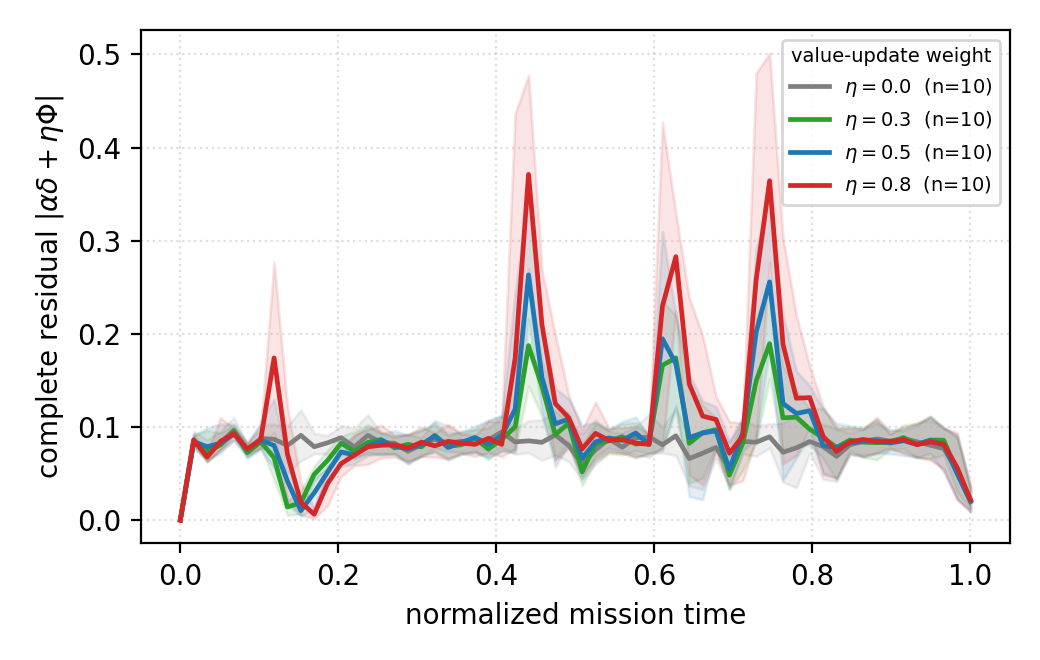
\includegraphics[width=\columnwidth]{qconv}
%% R2#9: "the band is inter-run spread rather than a confidence interval of the
%% mean... it might be worth stating in the caption rather than only in the text,
%% since readers often interpret such bands as inferential."
\caption{Complete update residual $|\alpha\delta+\eta\bm{\Phi}|$ over per-run series
resampled onto a common normalized-time grid, for $\eta\in\{0,0.3,0.5,0.8\}$
(configurations E0, E2, E3, E4). Each curve is the \emph{across-run mean}; the shaded
band is the $2.5$--$97.5$ \emph{percentile band of the per-run series}, that is, the
spread \emph{between runs}---it is \textbf{not} a confidence interval of the mean and
must not be read as one. The residual grows monotonically with $\eta$ while every
discrete behavioral metric is unchanged. For $\eta>0$ the residual is event-driven---flat between
events and spiking during each of the four reactive episodes (one hazard retreat and
three anomaly investigations) as $\eta\bm{\Phi}$ rises and decays, with the band widening
at the peaks---whereas for $\eta=0$ it stays near ${\approx}0.08$ between the
start-up transient and the end-of-mission decline, since the only term left is
$\alpha\delta$. Increments stay bounded (end-of-mission
${\approx}0.020$). The early region ($\lesssim0.2$ normalized time) mixes the
start-up transient with the retreat episode and the across-run alignment there is
loose; we draw no reading from it.}
\label{fig:qconv}
\end{figure}

\paragraph*{The update is affected by $\eta$; the behavior is not}
%% R2#4 pediu que a estabilidade do update fosse atestada no resíduo COMPLETO.
%% A Fig. com sobreposição de eta mostra que o instrumento detecta o termo que
%% deveria detectar -- e que o comportamento não o acompanha. É a afirmação
%% honesta disponível: o update está implementado como especificado e é estável,
%% e nada além disso.
Fig.~\ref{fig:qconv} overlays the complete update residual
$|\alpha\delta+\eta\Phi|$ for $\eta\in\{0,0.3,0.5,0.8\}$. The residual rises
monotonically with $\eta$---peak of the across-run mean $0.097$, $0.189$, $0.263$ and
$0.371$ respectively, with the per-run area under the curve separating completely
between $\eta=0$ and every $\eta>0$ (Cliff's $\delta=1.0$)---while every discrete
behavioral metric is unchanged. This is the expected arithmetic: the residual
contains $\eta\Phi$ by construction, so its growth with $\eta$ is close to
tautological. What the figure establishes is narrower and is all we claim: the update
is implemented as specified and its increments remain bounded and stable over the
mission, and the invariance of behavior is not an artifact of the term being inert in
the table. It says nothing about behavior, which is governed elsewhere.


\section*{Acknowledgment}
The conceptual diagrams in Figs.~\ref{fig:concept}--\ref{fig:fsm} and the
graphical abstract were rendered with the assistance of the AI-based
illustration tool Illustrae.CO from specifications authored by the authors. The authors also used a large language
model (Anthropic Claude) to assist in drafting and editing portions of the
manuscript text and the evaluation and analysis scripts. All AI-assisted content
was reviewed, verified, and edited by the authors, who take full responsibility
for the contents of this article. The quantitative figures
(Figs.~\ref{fig:world}, \ref{fig:box}, \ref{fig:traj}, and \ref{fig:qconv}) and
all experimental data were produced by the authors' own software without the use
of generative AI.

\bibliographystyle{IEEEtran}
\bibliography{references}

\begin{IEEEbiographynophoto}{Milton Miranda Neto}
received the B.S. degree in computer science from the Centro Universit\'ario do
Tri\^angulo (Unitri), Uberl\^andia, Brazil, in 1998, and the M.S. degree in
electrical engineering from the Universidade Federal de Uberl\^andia (UFU),
Uberl\^andia, in 2016, where he is currently pursuing the Ph.D. degree in
electrical engineering. He is a higher-education course coordinator and a
professor with the Universidade do Estado de Minas Gerais (UEMG) and the Centro
Universit\'ario do Tri\^angulo, and a researcher with CGWorks. His research
interests include computer graphics, virtual and augmented reality, the Internet
of Things, autonomous navigation, robotics, and artificial intelligence applied
to engineering.
\end{IEEEbiographynophoto}

\begin{IEEEbiographynophoto}{Alexandre Cardoso}
received the Ph.D. degree in electrical engineering from the University of
S\~ao Paulo (USP), S\~ao Paulo, Brazil, in 2002. He is currently a Full
Professor with the Faculty of Electrical Engineering, Universidade Federal de
Uberl\^andia (UFU), Uberl\^andia, Brazil. His research interests include virtual and augmented
reality, computer graphics, and their application to engineering, education, and
industrial systems.
\end{IEEEbiographynophoto}

\EOD
\end{document}
